\documentclass[a4paper,12pt,oneside]{article}

% Imported packages
\usepackage[english]{babel}
\usepackage[T1]{fontenc}
\usepackage[utf8]{inputenc}
\usepackage{amssymb}
\usepackage{amsmath}
\usepackage{bm}
\usepackage{listings}
\usepackage{graphicx}
\usepackage{geometry}
\usepackage{float}
\usepackage{subfigure}
\usepackage{wrapfig}
\usepackage{comment}
\usepackage{hyperref}

% Margin dimensions settings
\geometry{a4paper,top=2cm,bottom=2cm,left=2cm,right=2cm,%
heightrounded,bindingoffset=5mm}

% Enumeration settings
\renewcommand\thesubsection{\thesection.\alph{subsection}}

% Code visualization settings
\lstset{basicstyle=\small\ttfamily}

% Code design settings
\lstset{language=Matlab}

% Included images path
\graphicspath{{Images/}}

% Document information
\title{Fundamentals of Vibration Analysis and Vibroacoustics \\
Module 1 - Fundamentals of Vibration Analysis \\
Assignment 2 - Multi-degree-of-freedom systems}
\author{Bombaci Nicola 10677942 \\
Fantin Jacopo 10591775 \\
Intagliata Emanuele 10544878}
\date{May 2020}


\begin{document}

\maketitle

\vspace{30pt}

\section*{System schematic and parameters}

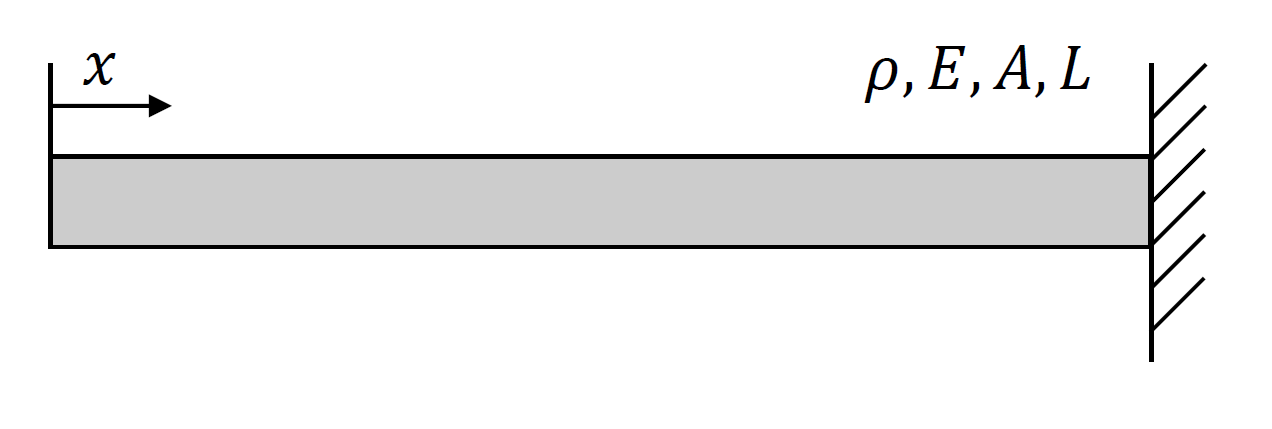
\includegraphics[width=0.9\textwidth]{system_schematic}

\vspace{30pt}

\begin{minipage}{0.4\textwidth}
	\[ \begin{split}
		& \begin{cases}
			M_1 = 5 \, \text{kg} \quad \text{,} \quad
				J_1 = 2.5 \, \text{kg m $ \! \! ^2 $} \\
			M_2 = 1.25 \, \text{kg} \quad \text{,} \quad
				J_2 = 0.16 \, \text{kg m $ \! \! ^2 $} \\
			M_3 = 10 \, \text{kg}
		\end{cases} \\[20pt]
		& \begin{cases}
			k_1 = 1000 \, \text{N/m} \\
			k_2 = 100 \, \text{N/m} \\
			k_3 = 560 \, \text{N/m} \\
			k_4 = 800 \, \text{N/m}
		\end{cases} \\[30pt]
	\end{split} \]
\end{minipage}
\begin{minipage}{0.4\textwidth}
\vspace{-20pt}
	\[ \begin{split}
		& \begin{cases}
			R_1 = 1 \, \text{m} \\
			R_2 = 0.5 \, \text{m}
		\end{cases} \\[25pt]
		& \begin{cases}
			c_1 = 0.5 \, \text{Ns/m} \\
			c_2 = 0.5 \, \text{Ns/m} \\
			c_3 = 1 \, \text{Ns/m} \\
			c_4 = 4 \, \text{Ns/m}
		\end{cases}
	\end{split} \]
\end{minipage}

\clearpage

\section{Equation of motion}

As a preliminary step, a reference system and sign conventions must be fixed. We chose to follow the commonly employed cartesian axes system, the counterclockwise rotation as the positive one and the spring elongation as the positive variation of the spring length:

\begin{figure}[H]
	\centering
	\subfigure{
		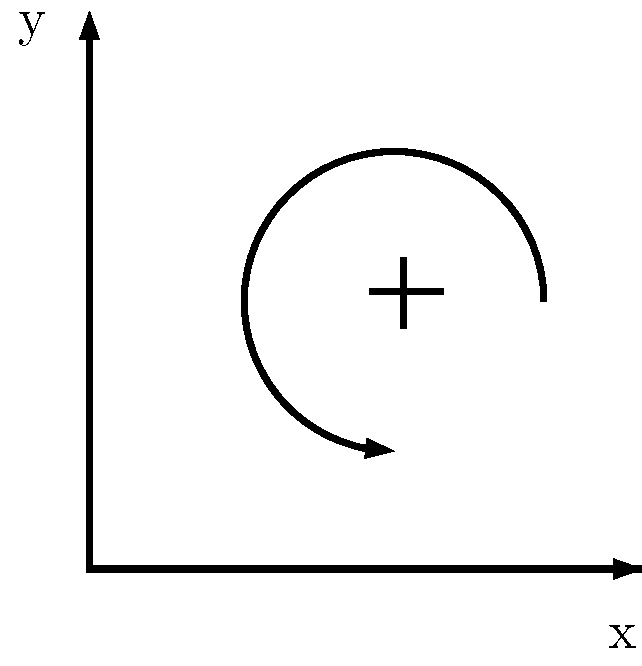
\includegraphics[width=0.15\linewidth]{reference_axes}}
	\hspace{50pt}
	\subfigure{
		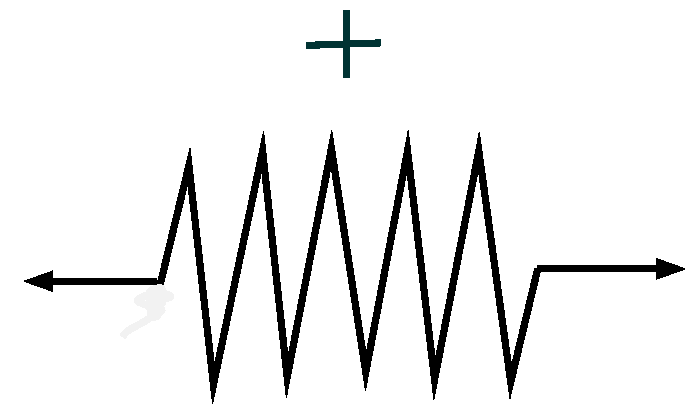
\includegraphics[width=0.15\linewidth]{reference_spring}}
\end{figure}

\subsection{Equation derivation}

\subsubsection*{Step 1: number of degrees of freedom identification}

We proceeded computing the number of degrees of freedom $ N $ of the system using the same computation as for Assignment 1:

\[ \begin{split}
	N = n_\textup{b} \cdot 3 ~ \text{DOF} = 9 ~ \text{DOF} & - \\
	1 ~ \text{DOF} & - \quad \text{(roller on point A)} \\
	2 ~ \text{DOF}  & - \quad \text{(2 rollers for body 3)} \\
	1 ~ \text{DOF} & - \quad \text{(string)} \\
	2 ~ \text{DOF} & = \quad \text{(bar)} \\
	3 ~ \text{DOF}
\end{split} \]

where $ n_\textup{b} $ is the number of bodies in the system, $ n_\textup{b} = 3 $ in this case. We chose to solve the problem directly using Lagrange equation, resulting in one equation per independent variable, so three equations only. We chose the rotations $ \theta_1 $ and $ \theta_2 $ of bodies 1 and 2 respectively and the horizontal displacement $ x_3 $ of body 3 as the independent variables for our analysis. These are gathered together into the independent variables vector $ \mathbf{u} = \begin{bmatrix} \theta_1 \\ \theta_2 \\ x_3 \end{bmatrix} $.

\subsubsection*{Step 2: energy terms definition}
\label{ssubs:energy_terms}

\[
	E_\textup{k} = \frac{1}{2} \, J_1 \, \omega_1^2 + \frac{1}{2} \, M_1 \, v_1^2 +
		\frac{1}{2} \, J_2 \, \omega_2^2 + \frac{1}{2} \, M_2 \, v_2^2 +
		\frac{1}{2} \, M_3 \, v_3^2
\]

Gravitational contributions are not taken into account since none of the bodies can move in the vertical direction because of the system constraints:

\[
	V = V_\textup{e} = \frac{1}{2} \, k_1 \, \Delta l_1^2 +
		\frac{1}{2} \, k_2 \, \Delta l_2^2 +
		\frac{1}{2} \, k_3 \, \Delta l_3^2 +
		\frac{1}{2} \, k_4 \, \Delta l_4^2
\]

\[
	D = \frac{1}{2} \, c_1 \, \dot{\Delta l_1}^2 +
		\frac{1}{2} \, c_2 \, \dot{\Delta l_2}^2 +
		\frac{1}{2} \, c_3 \, \dot{\Delta l_3}^2 +
		\frac{1}{2} \, c_4 \, \dot{\Delta l_4}^2
\]

Because the assignment's requests define external forces to compute the system's forced motion later on, we're assuming a horizontal force $ F(t) $, directed rightward, applied on point $ A $:

\[ \delta W = F(t) \, \delta x_\textup{F} \]

\subsubsection*{Step 3: physical variables as functions of independent ones}
\label{ssubs:jacobians}

What we need now are the Jacobian matrices that allow to pass from physical coordinates to independent ones.

\vspace{30pt}
\begin{minipage}{0.4\textwidth}
	$ \begin{array}{c||c|c|c}
							& \dot{\theta_1}	& \dot{\theta_2}	& \dot{x_3} \\
		\hline \hline
		v_1 			& 0								& R_2							& 1 \\
		\hline
		\omega_1 	& 1								& 0								& 0 \\
		\hline
		v_2				& 0								& 0								& 1 \\
		\hline
		\omega_2	& 0								& 1								& 0 \\
		\hline
		v_3				& 0								& 0								& 1
	\end{array} $
\end{minipage}
\begin{minipage}{0.1\textwidth}
	$ \Longrightarrow $
\end{minipage}
\begin{minipage}{0.5\textwidth}
	\[
		\mathbf{\Lambda_m} =
		\begin{bmatrix}
			0	& R_2	& 1 \\
			1	& 0		& 0 \\
			0	& 0		& 1 \\
			0	& 1		& 0 \\
			0	& 0		& 1
		\end{bmatrix}
	\]
\end{minipage}

\vspace{30pt}

\begin{minipage}{0.4\textwidth}
	$ \begin{array}{c||c|c|c}
								& \theta_1	& \theta_2	& x_3 \\
		\hline \hline
		\Delta l_1	&	0					&	-R_2			& -1 \\
		\hline
		\Delta l_2	&	-R_1			&	2 \, R_2	& 0 \\
		\hline
		\Delta l_3	&	R_1				&	R_2				& 0 \\
		\hline
		\Delta l_4	&	0					&	0					& 1
	\end{array} $
\end{minipage}
\begin{minipage}{0.1\textwidth}
	$ \Longrightarrow $
\end{minipage}
\begin{minipage}{0.5\textwidth}
	\[
		\mathbf{\Lambda_k} =
		\begin{bmatrix}
			0			& -R_2			& -1 \\
			-R_1	& 2 \, R_2	& 0 \\
			R_1		& R_2				& 0 \\
			0			& 0					& 1
		\end{bmatrix}
	\]
\end{minipage}

\vspace{30pt}

\begin{minipage}{0.4\textwidth}
	$ \begin{array}{c||c|c|c}
										& \theta_1	& \theta_2	& x_3 \\
		\hline \hline
		\delta x_F	&	0					&	R_2				& 1
	\end{array} $
\end{minipage}
\begin{minipage}{0.1\textwidth}
	$ \Longrightarrow $
\end{minipage}
\begin{minipage}{0.5\textwidth}
	\[
		\mathbf{\Lambda_F} =
		\begin{bmatrix}
			0	& R_2	& 1
		\end{bmatrix}
	\]
\end{minipage}

\vspace{40pt}

\subsubsection*{Step 4: resulting equation}

Remembering that the relationship between physical variables and independent ones is given by the Jacobians we found, we may write the Lagrangian component and the resulting motion equations (which are going to be three, as we have three independent variables) in matricial form as follows.

\[ \begin{split}
	& \delta W = \mathbf{Q_u}^\textup{T} \, \bm{\delta u} =
		F(t) \, \delta x_\textup{F} = F(t) \, \mathbf{\Lambda_F} \, \bm{\delta u}
		~ \Rightarrow ~ \mathbf{Q_u}^\textup{T} = F(t) \, \mathbf{\Lambda_F} =
		\begin{bmatrix}
			0	& F(t) \, R_2	& F(t)
		\end{bmatrix} \\
	& \Rightarrow ~ \mathbf{Q_u} =	\begin{bmatrix}
																		0 \\
																		F(t) \, R_2 \\
																		F(t)
																	\end{bmatrix}
\end{split} \]


\begin{align}
\label{eqn:motion}
	\biggl(\frac{\partial}{\partial t}
		\Bigl(\frac{\partial E_\textup{k}}
		{\partial \dot{\mathbf{u}}}\Bigr)\biggr)^\textup{T} -
		\biggl(\frac{\partial E_\textup{k}}{\partial \mathbf{u}}\biggr)^\textup{T} +
		\biggl(\frac{\partial V}{\mathbf{u}}\biggr)^\textup{T} +
		\biggl(\frac{\partial D}{\partial \dot{\mathbf{u}}}\biggr)^\textup{T} & =
		\mathbf{Q_u} \notag \\
	\Rightarrow ~
		\underbrace{\mathbf{\Lambda_m}^\textup{T} \, \mathbf{M} \, \mathbf{\Lambda_m}}_
		{\substack{\text{generalized} \\ \text{mass matrix} \\
		\text{$ \mathbf{M^*} $}}} \, \ddot{\mathbf{u}} +
		\underbrace{\mathbf{\Lambda_k}^\textup{T} \, \mathbf{C} \,	\mathbf{\Lambda_k}}_
		{\substack{\text{generalized} \\ \text{damping matrix} \\
		\text{$ \mathbf{C^*} $}}} \, \dot{\mathbf{u}} +
		\underbrace{\mathbf{\Lambda_k}^\textup{T} \, \mathbf{K} \, \mathbf{\Lambda_k}}_
		{\substack{\text{generalized} \\ \text{stiffness matrix} \\
		\text{$ \mathbf{K^*} $}}} \, \mathbf{u} & =
		\underbrace{\mathbf{\Lambda_F}^\textup{T} \, F(t)}_
		{\substack{\text{generalized} \\ \text{forces vector} \\
		\text{$ \mathbf{Q_u} $}}}
\end{align}

\subsection{Eigenfrequencies and eigenvectors}

We're asked to solve two eigenvalues-eigenvectors problem, one for the undamped system and one for the damped one. The to-be-found natural and damped natural eigenfrequencies of each mode of oscillation correspond, respectively, to the eigenvalues of the state matrices $ \mathbf{A_{und}} $ and $ \mathbf{A_d} $ of the undamped and damped system's characteristic equation, while the mode shapes to their eigenvectors, again both for undamped and damped case. The characteristic equation stems from the equation of motion where the external generalized forces term has been set equal to zero, i.e. analyzing the free motion of the system:

\[
	\mathbf{M^*} \, \ddot{\mathbf{u}} + \mathbf{C^*} \, \dot{\mathbf{u}} +
		\mathbf{K^*} \, \mathbf{u} = \mathbf{0}
\]

For both the undamped and damped case, we made use of the Matlab function \lstinline!eig()! passing $ \mathbf{A_{und}} $ and $ \mathbf{A_d} $ as parameters, which are, again, the state matrices of the undamped and damped system we're gonna see more in detail now.

\subsubsection*{Undamped case}
\label{ssubs:undamped_parameters}

In this case, the characteristic equation we obtain has no generalized damping matrix in it:

\[ (\gamma^2 \, \mathbf{M^*} + \mathbf{K^*}) \, \mathbf{U} = \mathbf{0} \]

where $ \gamma $ is the coefficient of time variable in the differential equation solution $ \mathbf{u} = \mathbf{U} \, e^{\gamma \, t} $. The reference eigenvalues-eigenvectors problem is ascribable to the standard problem:

\[ (\lambda \, \mathbf{I} - \mathbf{A_{und}}) \, \mathbf{x} = \mathbf{0} \]

So the state matrix $ \mathbf{A_{und}} $ in this case is

\[ \mathbf{A_{und}} = - \mathbf{M^{*^{-1}}} \, \mathbf{K^*} \]

This yields the following natural eigenfrequencies and undamped mode shapes (normalized with respect to the first element), one for each of the three modes:

\vspace{20pt}
\begin{minipage}{0.5\textwidth}
	1\textsuperscript{st} mode:
	\[
		\omega_\textup{n}^{(1)} = 9.7840 \, \text{rad/s} \hspace{20pt}
			\mathbf{U_{und}^{(1)}} =	\begin{bmatrix}
														1 \\
														-2.3371 \\
														2.4924
													\end{bmatrix}
	\]
\end{minipage}
\begin{minipage}{0.5\textwidth}
	2\textsuperscript{nd} mode:
	\[
		\omega_\textup{n}^{(2)} = 14.1841 \, \text{rad/s} \hspace{20pt}
			\mathbf{U_{und}^{(2)}} =	\begin{bmatrix}
														1 \\
														-0.8724 \\
														0.0018
													\end{bmatrix}
	\]
\end{minipage}

\vspace{5pt}

\begin{center}
	3\textsuperscript{rd} mode:
\end{center}
\[
	\omega_\textup{n}^{(3)} = 21.1479 \, \text{rad/s} \hspace{20pt}
		\mathbf{U_{und}^{(3)}} =	\begin{bmatrix}
													1 \\
													2.5449 \\
													-0.2877
												\end{bmatrix}
\]

As damping is being neglected, all the values in the eigenvectors are real.

\subsubsection*{Damped case}
\label{ssubs:damped_parameters}

The construction of the state matrix for the damped case is not as trivial as for the undamped case: we resort to the state-space representation.

\[ \begin{split}
	\mathbf{M^*} \, \ddot{\mathbf{u}} + \mathbf{C^*} \, \dot{\mathbf{u}} +
		\mathbf{K^*} \, \mathbf{u} = \mathbf{0} \\[10pt]
	\Rightarrow ~ \begin{bmatrix}
									\mathbf{M^*}	& \mathbf{0} \\
									\mathbf{0}		& \mathbf{M^*}
								\end{bmatrix}
								\begin{bmatrix}
									\ddot{\mathbf{u}} \\
									\dot{\mathbf{u}}
								\end{bmatrix} =
								\begin{bmatrix}
									- \mathbf{C^*}	& - \mathbf{K^*} \\
									\mathbf{M^*}		& \mathbf{0}
								\end{bmatrix}
								\begin{bmatrix}
									\dot{\mathbf{u}} \\
									\mathbf{u}
								\end{bmatrix} \\[10pt]
	~ \Rightarrow \mathbf{A_d} =	\begin{bmatrix}
																	\mathbf{M^*}	& \mathbf{0} \\
																	\mathbf{0}		& \mathbf{M^*}
																\end{bmatrix}^{-1}
																\begin{bmatrix}
																	- \mathbf{C^*}	& - \mathbf{K^*} \\
																	\mathbf{M^*}		& \mathbf{0}
																\end{bmatrix}
\end{split} \]

\clearpage

This leads to the damping factor, damped frequency and normalized damped mode shape for each mode:

\vspace{10pt}

1\textsuperscript{st} mode:
\[
	\alpha^{(1)} = 0.1910 \, \text{rad/s} \hspace{20pt}
		\omega_\textup{d}^{(1)} = 9.7838 \, \text{rad/s} \hspace{20pt}
		\mathbf{U_d^{(1)}} =	\begin{bmatrix}
													1 \\
													-2.3361 - j0.0296 \\
													2.4856 + j0.1356
												\end{bmatrix}
\]

2\textsuperscript{nd} mode:
\[
	\alpha^{(2)} = 0.3036 \, \text{rad/s} \hspace{20pt}
		\omega_\textup{d}^{(2)} = 14.1792 \, \text{rad/s} \hspace{20pt}
		\mathbf{U_d^{(2)}} =	\begin{bmatrix}
													1 \\
													-0.8731 + j0.0014 \\
													0.0020 + j0.0106
												\end{bmatrix}
\]

3\textsuperscript{rd} mode:
\[
	\alpha^{(3)} = 0.3850 \, \text{rad/s} \hspace{20pt}
		\omega_\textup{d}^{(3)} = 21.1432 \, \text{rad/s} \hspace{20pt}
		\mathbf{U_d^{(3)}} =	\begin{bmatrix}
													1 \\
													2.5433 + j0.0499 \\
													-0.2874 -j0.0132
												\end{bmatrix}
\]

It's worth it to say the damped eigenfrequencies are very much close to the undamped ones, as the damping is light enough, and the eigenvectors are now complex, as damping has been introduced.

\subsection{Proportional damping matrix}
\label{subs:rayleigh_damping}

In place of the generalized damping matrix $ \mathbf{C^*} $, we may as well use a matrix $ \mathbf{C_{ray}} $ that approximates it using the Rayleigh proportional damping, that is a linear combination of the generalized mass and stiffness matrices through coefficients $ \alpha_\textup{ray} $ and $ \beta_\textup{ray} $:

\[
	\mathbf{C_{ray}} =
		\alpha_\textup{ray} \, \mathbf{M^*} + \beta_\textup{ray} \, \mathbf{K^*}
\]

We started computing the damping ratios $ \xi_i $ as $ \frac{C^*_{ii}}{C^*_{\textup{cr}_{ii}}} = \frac{C^*_{ii}}{2 \, M^*_{ii} \, \omega_\textup{n}^{(i)}} $ for $ i = 1, 2, 3 $, stored in the vector $ \bm{\xi} $, then exploited the relationship between the values of $ \bm{\xi} $ and $ \alpha_\textup{ray}, \beta_\textup{ray} $ obtained by substituting $ C^*_{ii} = \alpha_\textup{ray} \, M^*_{ii} + \beta_\textup{ray} \, K^*_{ii} $ in the expression for $ \xi_i $ in order for us to find the values of $ \alpha_\textup{ray} $ and $ \beta_\textup{ray} $:

\[ \begin{split}
	& \bm{\xi} =	\begin{bmatrix}
									\xi_1 \\
									\xi_2 \\
									\xi_3
								\end{bmatrix} =
		\begin{bmatrix}
		 	\frac{1}{\omega_\textup{n}^{(1)}}	& \frac{\omega_\textup{n}^{(1)}}{2} \\
			\frac{1}{\omega_\textup{n}^{(2)}}	& \frac{\omega_\textup{n}^{(2)}}{2} \\
			\frac{1}{\omega_\textup{n}^{(3)}}	& \frac{\omega_\textup{n}^{(3)}}{2}
		\end{bmatrix} \begin{bmatrix}
										\alpha_\textup{ray} \\
										\beta_\textup{ray}
									\end{bmatrix} ~ \Rightarrow ~
		\begin{bmatrix}
			\alpha_\textup{ray} \\
			\beta_\textup{ray}
		\end{bmatrix} =
		\begin{bmatrix}
			\frac{1}{\omega_\textup{n}^{(1)}}	& \frac{\omega_\textup{n}^{(1)}}{2} \\
			\frac{1}{\omega_\textup{n}^{(2)}}	& \frac{\omega_\textup{n}^{(2)}}{2} \\
			\frac{1}{\omega_\textup{n}^{(3)}}	& \frac{\omega_\textup{n}^{(3)}}{2}
		\end{bmatrix}^{-1}	\begin{bmatrix}
													\xi_1 \\
													\xi_2 \\
													\xi_3
												\end{bmatrix} = \begin{bmatrix}
																					0.7078 \\
																					-0.0008
																				\end{bmatrix} \\
	& \Rightarrow ~ \mathbf{C_{ray}} =	\begin{bmatrix}
																				1.2144	& -0.1514	& 0 \\
																				-0.1514	& 0.5858	& 1.3490 \\
																				0				& 1.3490	& 9.9881
																			\end{bmatrix}
\end{split} \]

where as the inverse of the 3x2 matrix we used the Matlab function \lstinline!pinv()! to compute its Moore-Penrose pseudoinverse. $ \mathbf{C_{ray}} $ is a symmetric matrix, as expected, as it's a linear combination of symmetric matrices. From now on, this just-found proportional damping matrix is going to be employed as the damping matrix for the system.


\section{Free motion of the system}
\label{sec:free_motion}

Like for the single-degree-of-freedom systems, the equation describing the free motion of each independent variable comes from solving the motion equation when no external forces or torques are acting. We already solved this equation in the previous steps, which allowed us to obtain the damping coefficients vector $ \bm{\alpha} $, the damped natural frequencies vector $ \bm{\omega_\textup{\textbf{d}}} $ and the damped mode shapes $ \mathbf{U_d} $:

\[ \begin{split}
	& \bm{\alpha} =	\begin{bmatrix}
									\alpha^{(1)} \\
									\alpha^{(2)} \\
									\alpha^{(3)}
								\end{bmatrix} = \begin{bmatrix}
																	0.1910 \\
																	0.3036 \\
																	0.3850
																\end{bmatrix} \hspace{50pt}
		\bm{\omega_\textup{\textbf{d}}} =	\begin{bmatrix}
																				\omega_\textup{d}^{(1)} \\
																				\omega_\textup{d}^{(2)} \\
																				\omega_\textup{d}^{(3)} \\
																			\end{bmatrix} = \begin{bmatrix}
																												9.7838 \\
																												14.1792 \\
																												21.1432
																											\end{bmatrix} \\
	& \mathbf{U_d} =	\begin{bmatrix}
											\mathbf{U_d^{(1)}}
											\mathbf{U_d^{(2)}}
											\mathbf{U_d^{(3)}}
										\end{bmatrix} =
		\begin{bmatrix}
			1									& 1									& 1 \\
			-2.3361 - j0.0296	& -0.8731 + j0.0014	& 2.5433 + j0.0499 \\
			2.4856 + j0.1356	& 0.0020 + j0.0106	& -0.2874 -j0.0132
		\end{bmatrix}
\end{split} \]

\subsection{Response to given initial conditions}
\label{subs:free_motion_given_initial_conditions}

We're now able to manually build the analytic expression for the free motion of each independent variable:

\[
	\mathbf{u^{free}}(t) =
		\sum_{i=1}^3 e^{-\alpha^{(i)} \, t} \, |\mathbf{U_d^{(i)}}|
		\Bigl(A^{(i)} \,
		\cos\bigl(\omega_\textup{d}^{(i)} \, t + \angle(\mathbf{U_d^{(i)}})\bigr) +
		B^{(i)} \,
		\sin\bigl(\omega_\textup{d}^{(i)} \, t + \angle(\mathbf{U_d^{(i)}})\bigr)\Bigr)
\]

Prior to that, the relationship between the given initial conditions for both position and velocity of each independent variable and the coefficients of each sinusoidal term in the free response must be extracted: we manually computed the derivative with respect to time of the equation relative to the free motion for each variable to obtain the velocities, then evaluated the two expressions at initial time $ t = 0 $ and set them to be equal to the initial conditions, factoring out each of the cosine coefficient $ A^{(i)} \, \text{, i=1,2,3} $ and each of the sine ones $ B^{(i)} $ and, by doing so, writing each initial condition as a linear combination of those coefficients. The coefficients of the linear combinations, depending on system parameters only, are gathered in the matrix called $ \mathbf{S} $:

\begin{align}
\label{eqn:coefficients_from_initial_conditions}
	& \begin{bmatrix}
			\mathbf{u_0} \\
			\dot{\mathbf{u}}_0
		\end{bmatrix} =
			\begin{bmatrix}
				\Re\{\mathbf{U_d}\} &	\Im\{\mathbf{U_d}\} \\
				-\bm{\alpha}^\textup{T} \circ \Re\{\mathbf{U_d}\} -
					\bm{\omega_\textup{\textbf{d}}}^\textup{T} \circ \Im\{\mathbf{U_d}\} &
					-\bm{\alpha}^\textup{T} \circ \Im\{\mathbf{U_d}\} +
					\bm{\omega_\textup{\textbf{d}}}^\textup{T} \circ \Re\{\mathbf{U_d}\}
			\end{bmatrix} \begin{bmatrix}
										\mathbf{A} \\
										\mathbf{B}
									\end{bmatrix} \notag \\[10pt]
	& \Rightarrow ~ \begin{bmatrix}
										\theta_{1_0} \\
										\theta_{2_0} \\
										x_{3_0}	\\
										\dot{\theta}_{1_0} \\
										\dot{\theta}_{2_0} \\
										\dot{x}_{3_0}
									\end{bmatrix} = \mathbf{S}	\begin{bmatrix}
																								A^{(1)} \\
																								A^{(2)} \\
																								A^{(3)} \\
																								B^{(1)}	\\
																								B^{(2)}	\\
																								B^{(3)}
																							\end{bmatrix} ~ \Rightarrow ~
		\begin{bmatrix}
			A^{(1)} \\
			A^{(2)} \\
			A^{(3)} \\
			B^{(1)}	\\
			B^{(2)}	\\
			B^{(3)}
		\end{bmatrix} = \mathbf{S}^{-1} \begin{bmatrix}
																			\theta_{1_0} \\
																			\theta_{2_0} \\
																			x_{3_0}	\\
																			\dot{\theta}_{1_0} \\
																			\dot{\theta}_{2_0} \\
																			\dot{x}_{3_0}
																		\end{bmatrix} =
		\begin{bmatrix}
			0.0065 \\
			0.2170 \\
			0.0382 \\
			0.0449 \\
			-0.0654 \\
			0.0565
		\end{bmatrix} \hspace{30pt}
		\text{with} \hspace{10pt} \begin{cases}
																\theta_{1_0} = \frac{\pi}{12} \, \text{rad} \\
																\theta_{2_0} = -\frac{\pi}{12} \, \text{rad} \\
																x_{3_0} = 0.1 \, \text{m} \\
																\dot{\theta}_{1_0} = 0.5 \, \text{rad/s} \\
																\dot{\theta}_{2_0} = 2 \, \text{rad/s} \\
																\dot{x}_{3_0} = 1 \, \text{m/s}
															\end{cases}
\end{align}

where the symbol $ \circ $ is the row-wise product. These values for elements for vectors $ \mathbf{A} $ and $ \mathbf{B} $ shows that these initial conditions excite all vibration modes, as no value is null, and without particularly favoring one mode over the others. To be sure the matrix $ \mathbf{S} $ has been correctly derived, the analytic solutions have been compared to the integrated ones obtained using the state matrix $ \mathbf{A_d} $ with Matlab \lstinline!ode45()! function:

\begin{lstlisting}
	odefun = @(t,y) A_damp*y;
	[t_ode,sol] = ode45(odefun,[t(1) t(end)],[u_0_dot;u_0]);
\end{lstlisting}

\vspace{10pt}

In the following plot, we show the response of the three variables to the given initial conditions both by making use of the $ \mathbf{S} $ matrix and by using the  \lstinline!ode45()! function. As we can see, the two perfectly coincide, validating our procedure. The most evident feature is that, while the two rotations are clearly a superposition of different modes and have a more chaotic motion, the displacement has a behavior very well approximated by the free motion of a single-degree-of-freedom system, meaning that, with these initial conditions that result in a quite uniform mixture of all three oscillation modes, one of these is prominent in terms of amplitude with respect to the other two, as for the third independent variable. From a very rough estimation, we may infer that this prominent mode is the first one, as the frequency is slightly higher than 3 cycles in the first 2 seconds, i.e. slightly higher than $ 1.5 \, \text{Hz} \approx 9.42 \, \text{rad/s} $, which corresponds to $ \omega_\textup{d}^{(1)} $. This could have been predicted assessing the modulus of the elements of the mode shapes relative to the third independent varaible: the one for the first mode shape is two orders of magnitude greater than the one for the second mode shape and one order of magnitude greater than the one for mode 3.

\begin{figure}[h]
	\hspace{-70pt}
	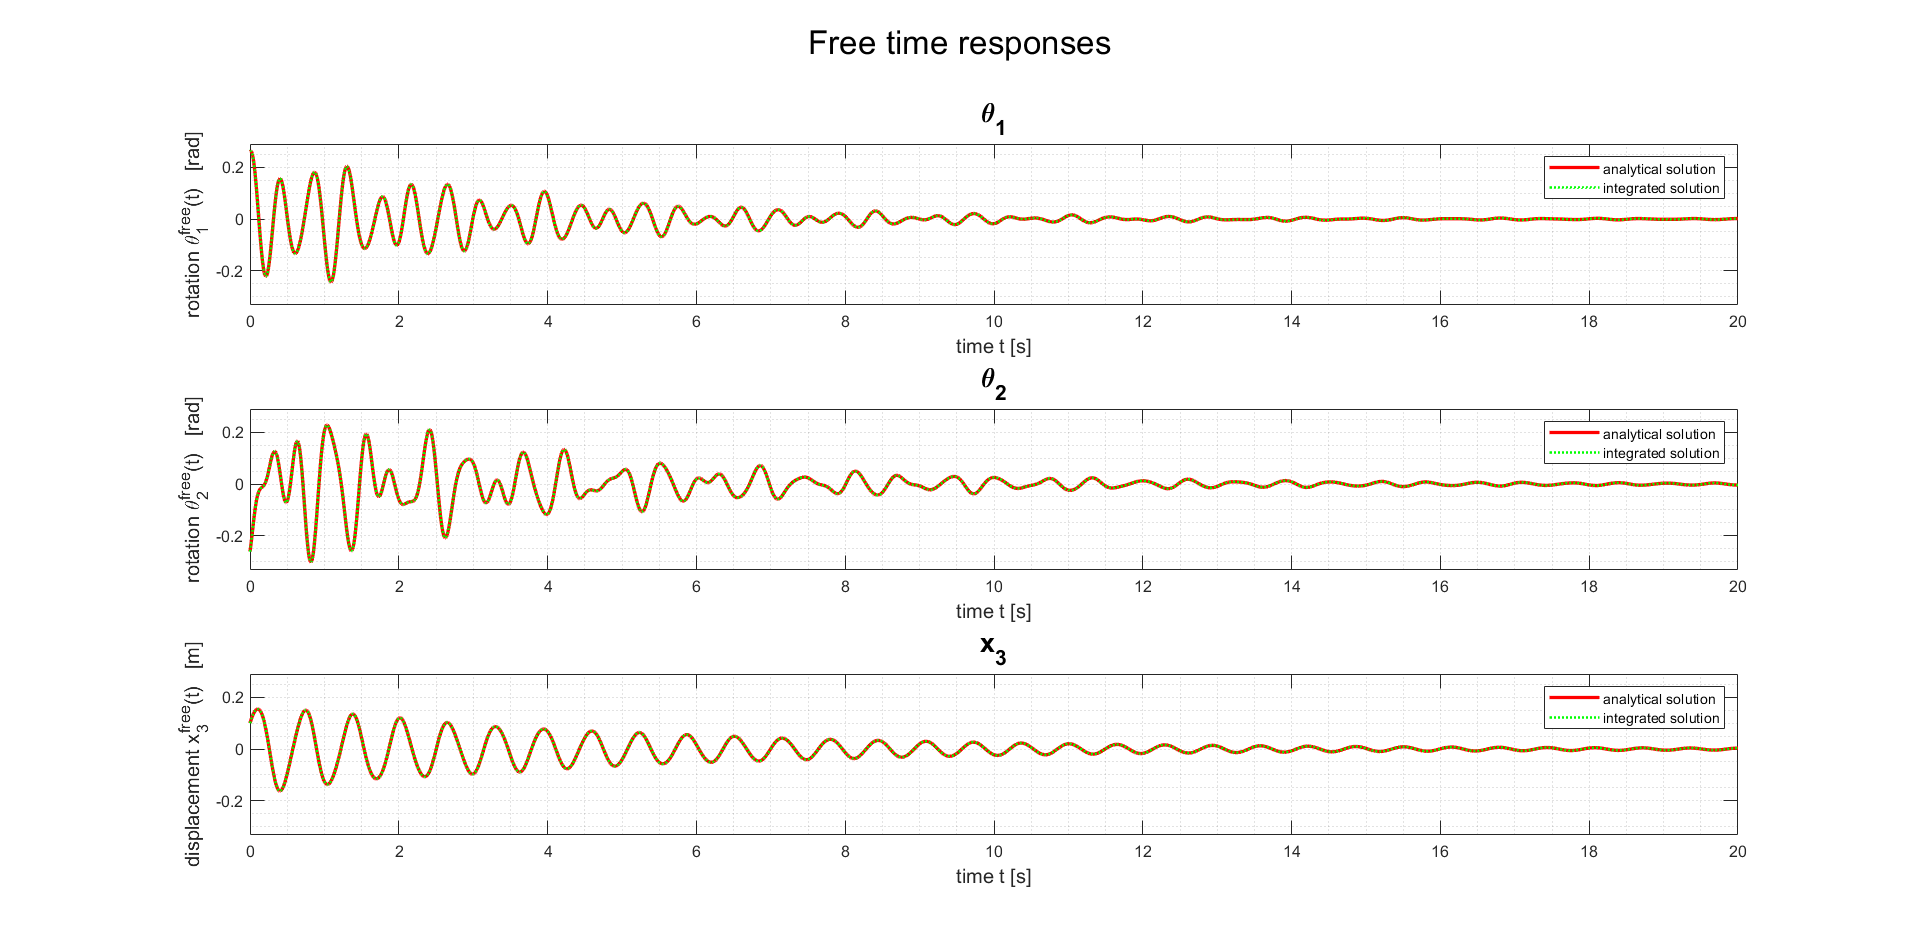
\includegraphics[scale=0.4]{free_time_responses}
\end{figure}

%\clearpage

\subsection{Exciting one mode only}
\label{subs:mode_2_excitation}

At this point, it's quite easy to set the initial conditions so that only one mode is going to show up in the free response: those are some initial conditions that make sure the $ A^{(i)} $ and $ B^{(i)} $ are different from zero for only one value of $ i $, and equal to zero for all the others. For example, willing to force the second mode only and with a unitary value for both the coefficients, we obtain

\[
	\mathbf{A} = \begin{bmatrix}
									A^{(1)} \\
									A^{(2)} \\
									A^{(3)}
								\end{bmatrix} = \mathbf{B} =	\begin{bmatrix}
																								B^{(1)} \\
																								B^{(2)} \\
																								B^{(3)}
																							\end{bmatrix} = \begin{bmatrix}
																																0 \\
																																1 \\
																																0
																															\end{bmatrix}
\]

We may then apply the direct formula in \eqref{eqn:coefficients_from_initial_conditions} to result in the initial conditions to be applied:

\[
	\begin{bmatrix}
		\theta_{1_0} \\
		\theta_{2_0} \\
		x_{3_0}	\\
		\dot{\theta}_{1_0} \\
		\dot{\theta}_{2_0} \\
		\dot{x}_{3_0}
	\end{bmatrix} = \mathbf{S}	\begin{bmatrix}
																A^{(1)} \\
																A^{(2)} \\
																A^{(3)} \\
																B^{(1)}	\\
																B^{(2)}	\\
																B^{(3)}
															\end{bmatrix} =
		\mathbf{S}	\begin{bmatrix}
									0 \\
									1 \\
									0 \\
									0 \\
									1 \\
									0
								\end{bmatrix} = \begin{bmatrix}
																	1 \\
																	-0,8716 \\
																	0.0126 \\
																	13.8756 \\
																	-12.1349 \\
																	-0.1252
																\end{bmatrix}
\]

\vspace{10pt}

The free responses obtained with these initial conditions are depicted in time domain in the following. In accordance with the fact only one mode is present, each variable oscillates with different initial phases and amplitudes, but at just one frequency and at the same decay rate. Moreover, the third independent variable is almost a constant at zero value when comparing it with the other two, indicating the third body stays almost still during this free motion: this means the second mode contributes extremely little to the overall motion of that body, in comparison with the other modes.

\begin{figure}[h]
	\hspace{-70pt}
	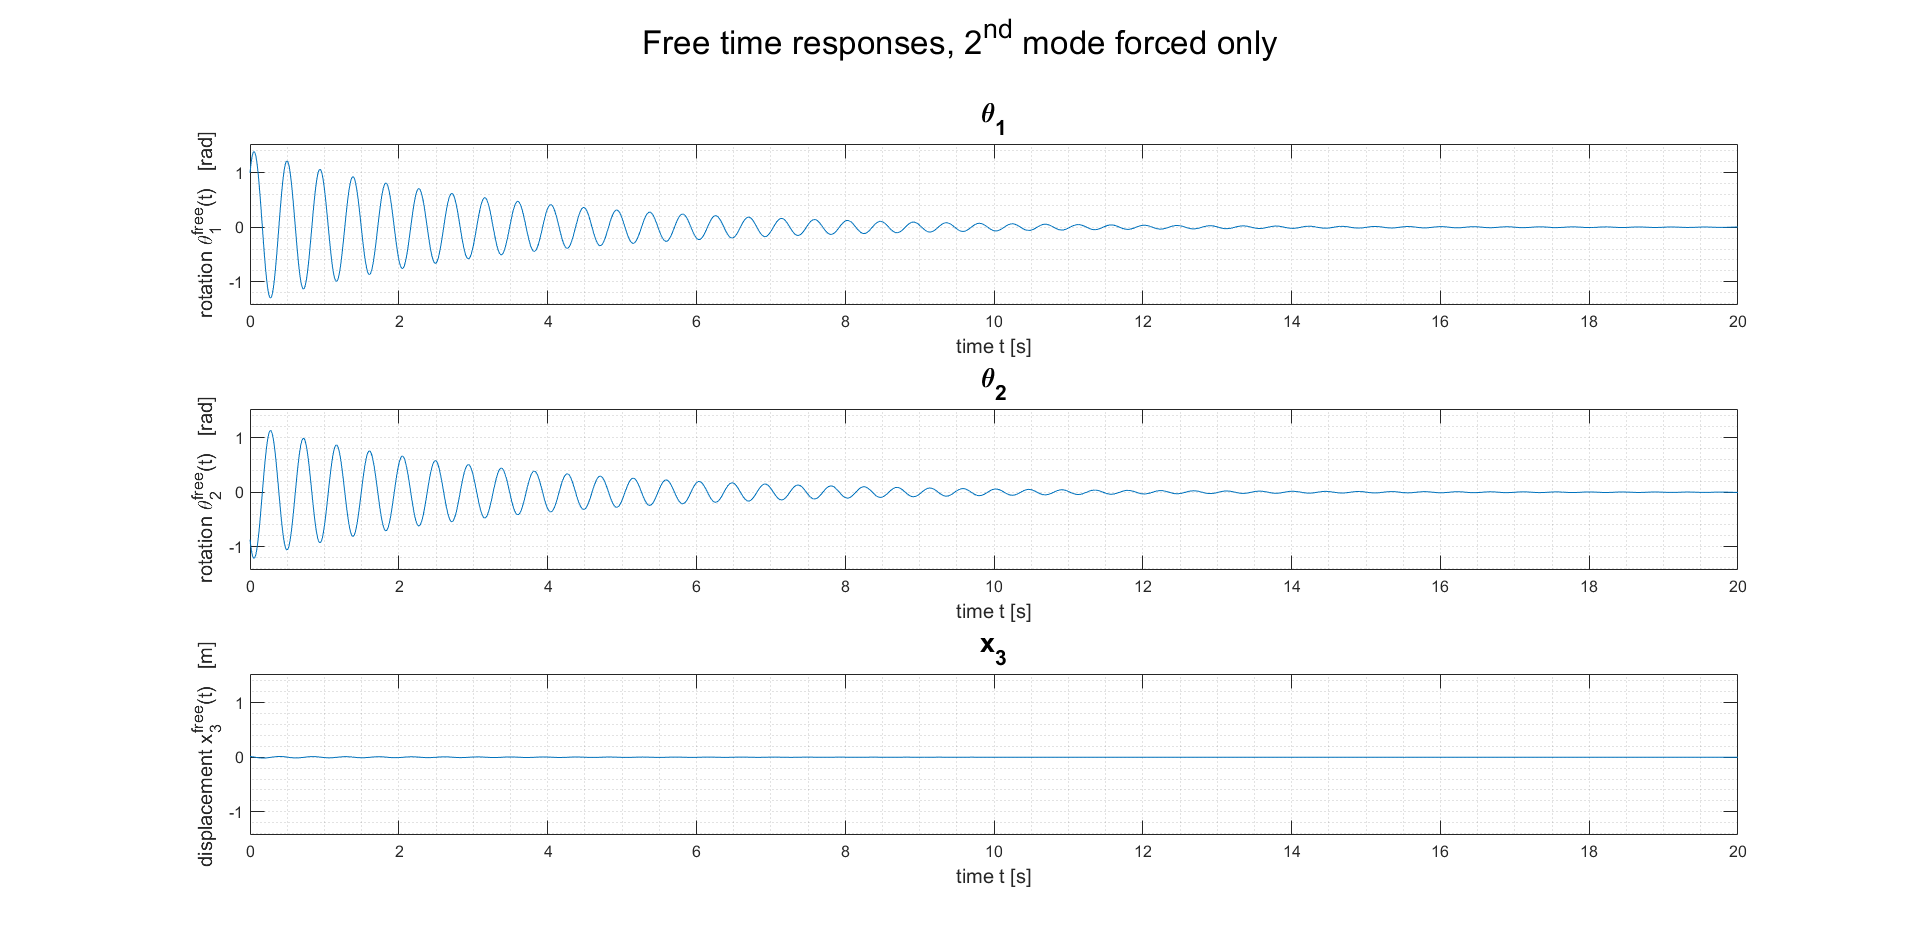
\includegraphics[scale=0.4]{free_time_responses_mode2}
\end{figure}

A zoomed view of the graph for the third independent variable is showed here: we may again appreciate the fact a single mode is present in the motion.

\clearpage

\begin{figure}[h]
	\hspace{-70pt}
	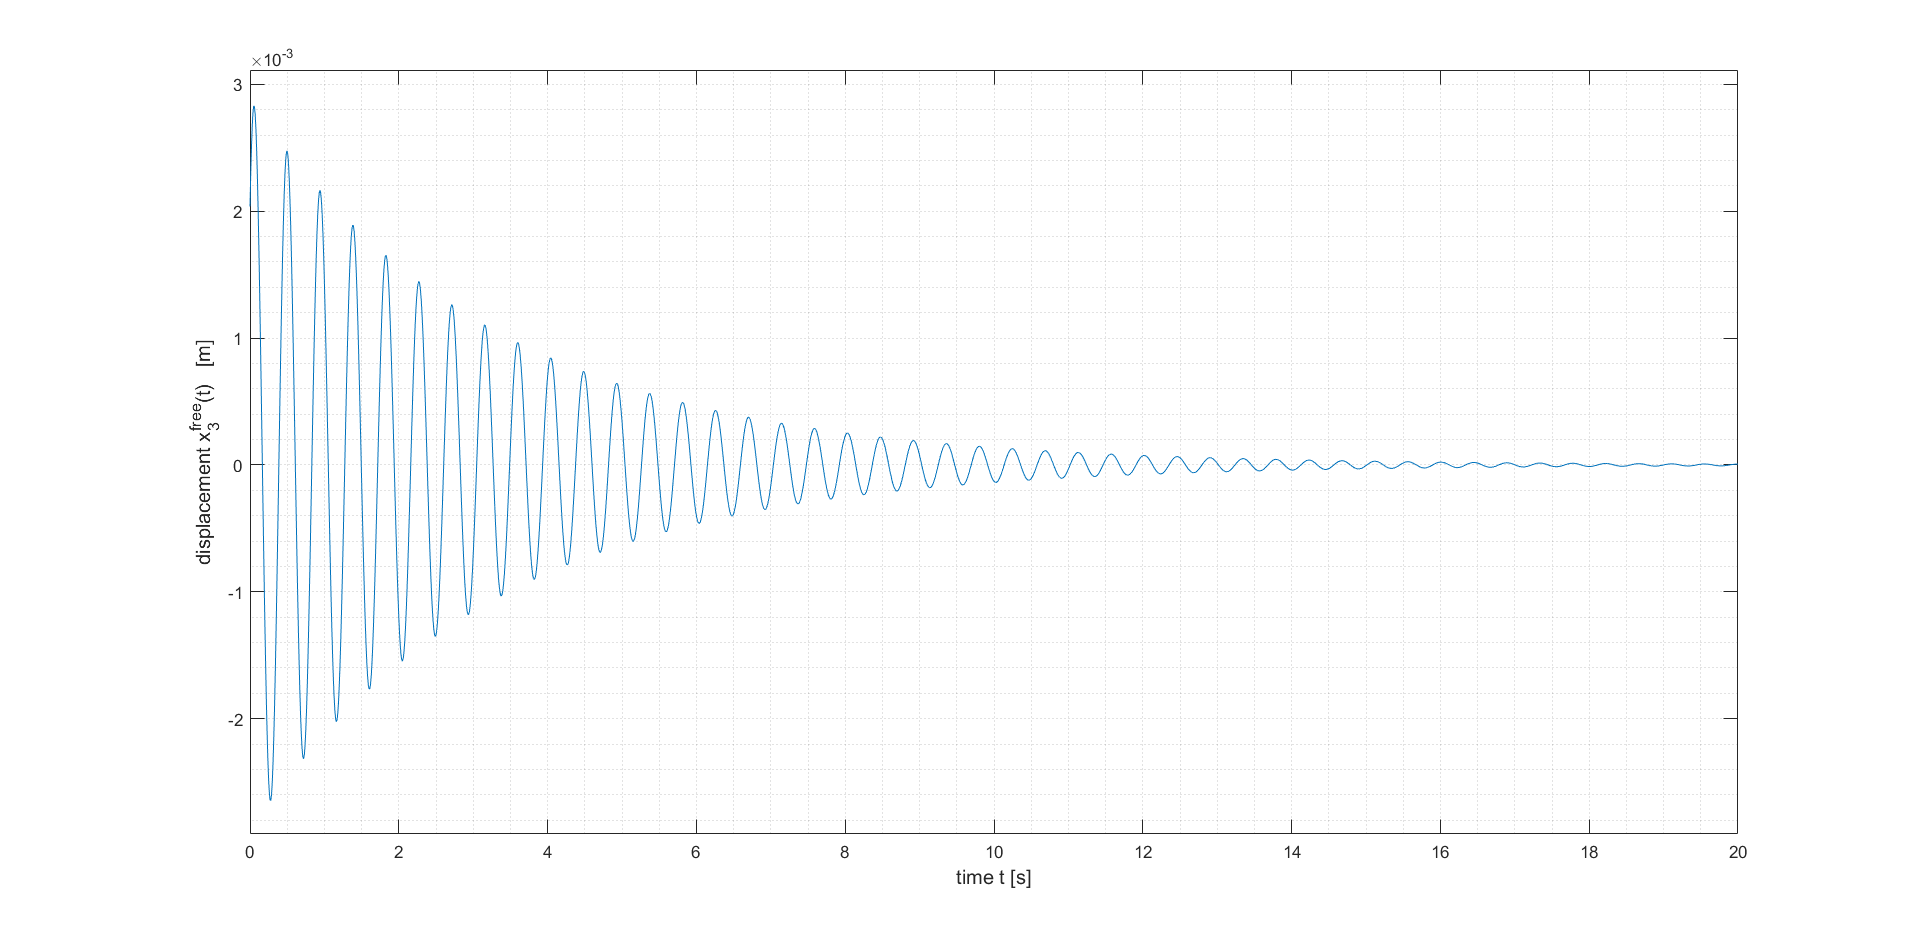
\includegraphics[scale=0.4]{free_time_responses_mode2_x3}
\end{figure}


\section{Forced motion of the system}

Considering the Rayleigh damping found in \ref{subs:rayleigh_damping}, we now study the forced motion of the system.

\subsection{Frequency Response Matrix}
\label{subs:frm}

Analogously to the considerations we made for the one-degree-of-freedom system, for computing the system's Frequency Response Functions we are implicitly considering one generalized force for each variable, such that each of them is applied to the body corresponding to that independent variable and has a Jacobian matrix of zeros except for a 1 in correspondence with that variable. The FRFs that we find applying the formula

\[
	\mathbf{H}(\Omega) = \mathbf{D}(\Omega)^{-1} =
		(- \Omega^2 \, \mathbf{M^*} + j \, \Omega \, \mathbf{C_{ray}} + \mathbf{K^*})^{-1}
\]

are, then, the transfer functions between each of the independent variables and each of these generalized forces. This way, we found a Frequency Response Matrix (FRM) where the element $ H_{ij}(\Omega) $ is the transfer function between the i-th independent variable and the j-th generalized force. Note that the FRFs appearing on the diagonal of the matrix are the co-located FRFs, meaning that they relate an independent variable to the correspondent generalized force.

\[
	\mathbf{H}(\Omega) = \begin{bmatrix}
								H_{11}(\Omega)	& H_{12}(\Omega)	& H_{13}(\Omega) \\
								H_{21}(\Omega)	& H_{22}(\Omega)	& H_{23}(\Omega) \\
								H_{31}(\Omega)	& H_{32}(\Omega)	& H_{33}(\Omega)
							\end{bmatrix}
\]

The corresponding plots in terms of magnitude and phase follow:

\begin{figure}[h]
	\hspace{-70pt}
	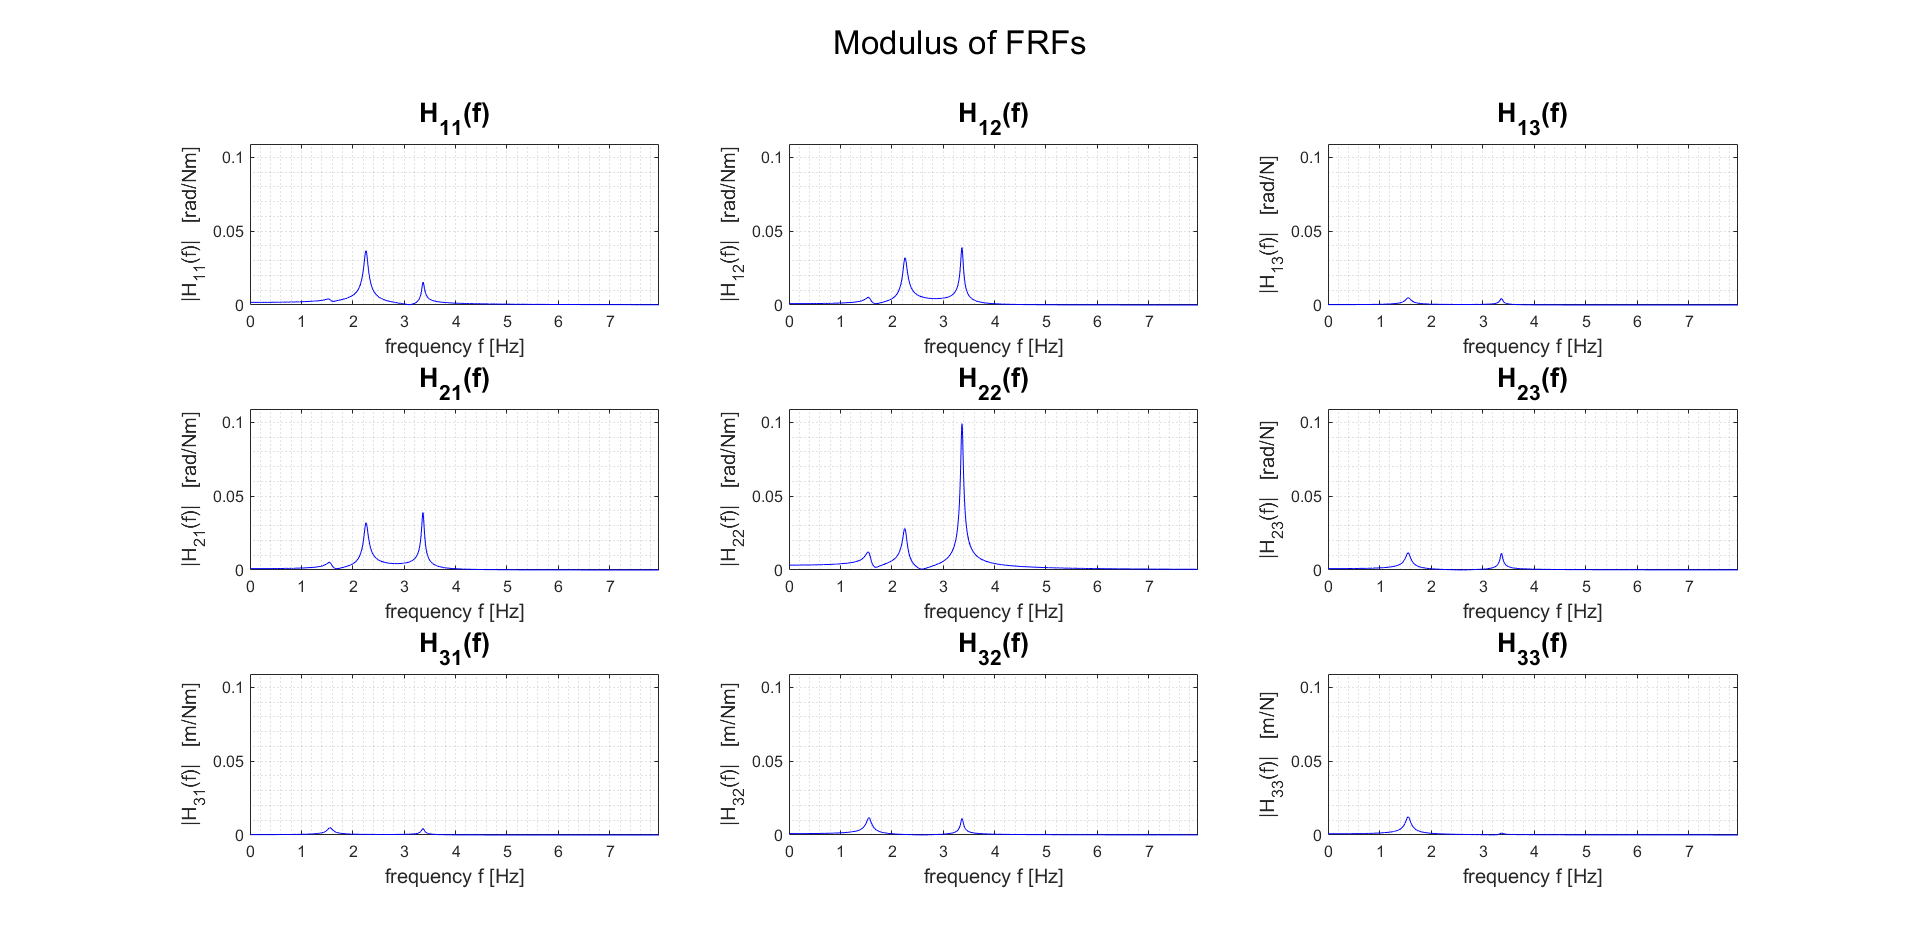
\includegraphics[scale=0.4]{frfs_modulus}
\end{figure}

\begin{figure}[H]
	\hspace{-70pt}
	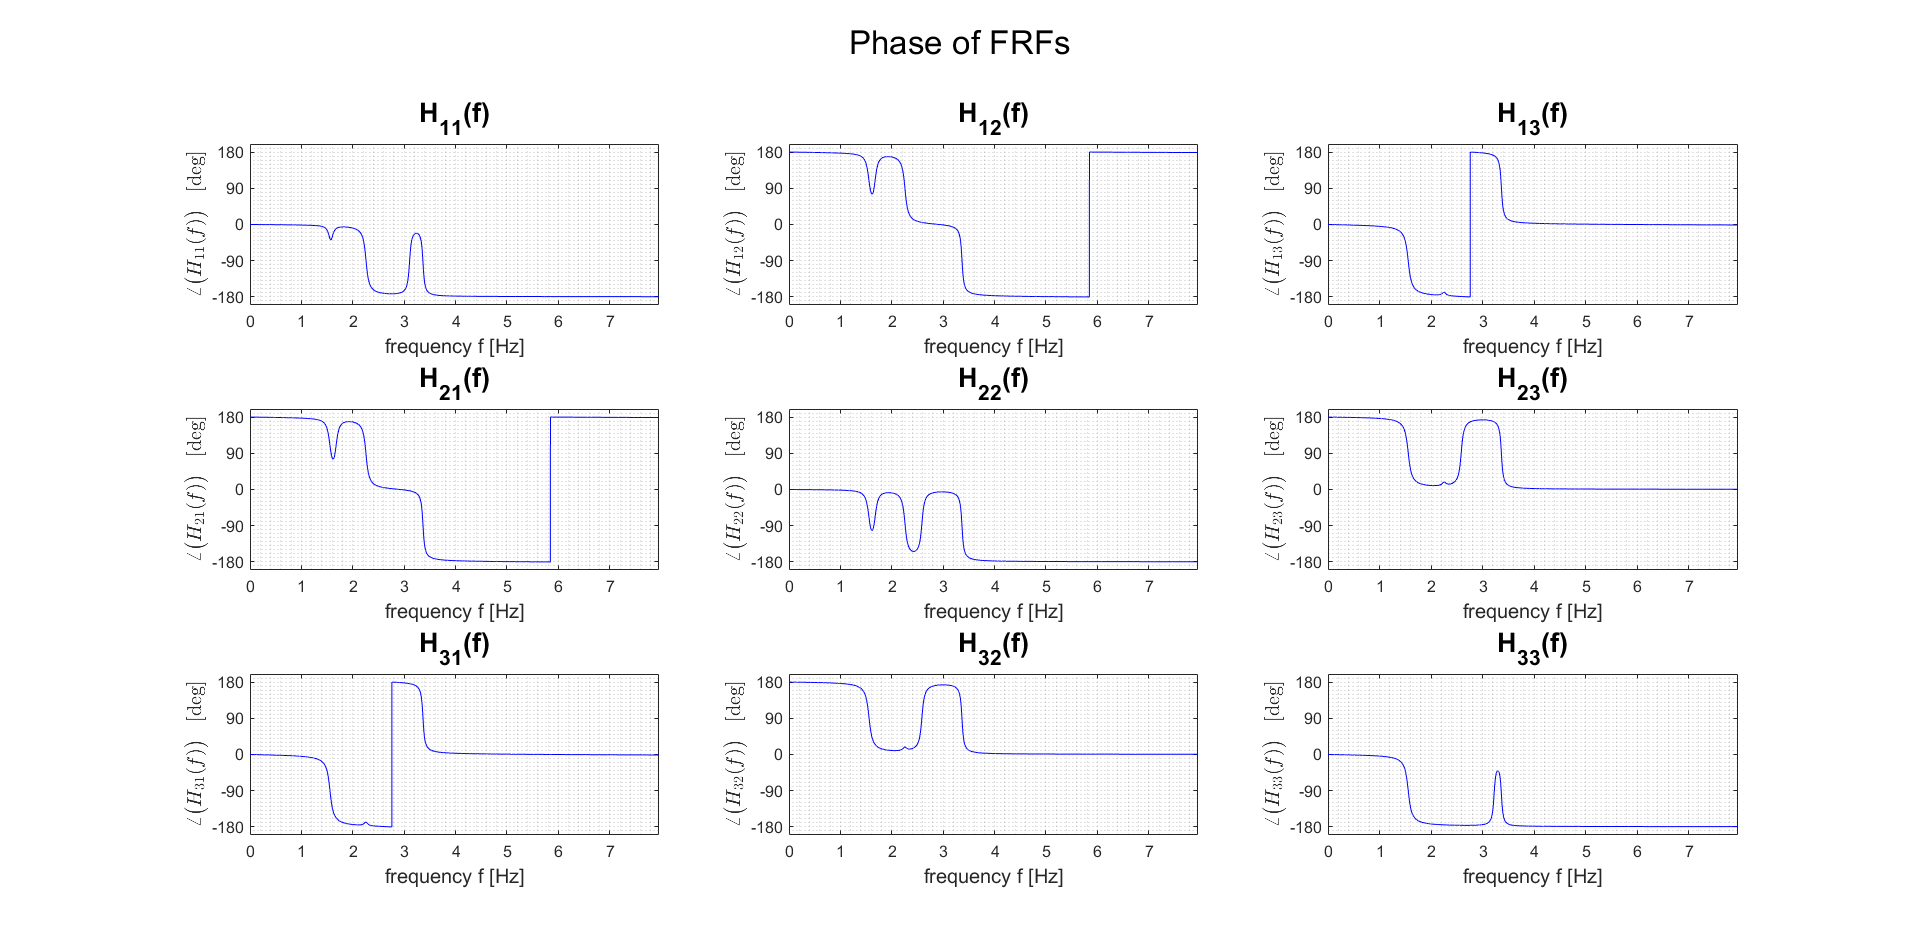
\includegraphics[scale=0.4]{frfs_phase}
\end{figure}

As expected, the matrix is symmetric, which also tells us that some sort of reciprocity principle holds: the same behavior is observed moving one body and observing another one or moving the latter and observing the former.

We immediately notice the displacement of the third body in resonance condition is by far smaller than the rotations of the two discs. We also see that the second mode is almost unperceivable in the displacement of body 3, which explains why $ x_3 $ has such a little oscillation with respect to $ \theta_1 $ and $ \theta_2 $ in \ref{subs:mode_2_excitation}. Here's a zoomed view of what happens in the FRF modulus matrix' last row: in correspondence with the second mode, it is barely possible to spot the small variations in the graphs. For $ H_{33}(\Omega) $, the second mode's peak doesn't even correspond to a flat curve portion like in $ H_{32}(\Omega) $, but only to a decrease in the graph's decreasing rate, i.e. to an increase in the function's first derivative or an inflection point.

\begin{figure}
	\hspace{-70pt}
	\includegraphics[scale=0.4]{frfs_x3}
\end{figure}

\subsection{Co-located FRF of point A}
\label{subs:co-located_a}

Let's now consider the system as we did in \eqref{eqn:motion}, with the external force applied to point $ A $, and let's retrieve the FRF between the displacement of point $ A $ itself and this force. In order to do so, the FRM must be multiplied by the Jacobian relative to the force computed at \ref{ssubs:jacobians}, which is already the force we're considering in this paragraph. So

\[
	H^\textup{coloc}_A(\Omega) =
		\mathbf{\Lambda_F} \, \mathbf{H}(\Omega) \, \mathbf{\Lambda_F}^\textup{T}
\]

which gives the following amplitude and phase diagrams.

\begin{figure}[H]
	\hspace{-70pt}
	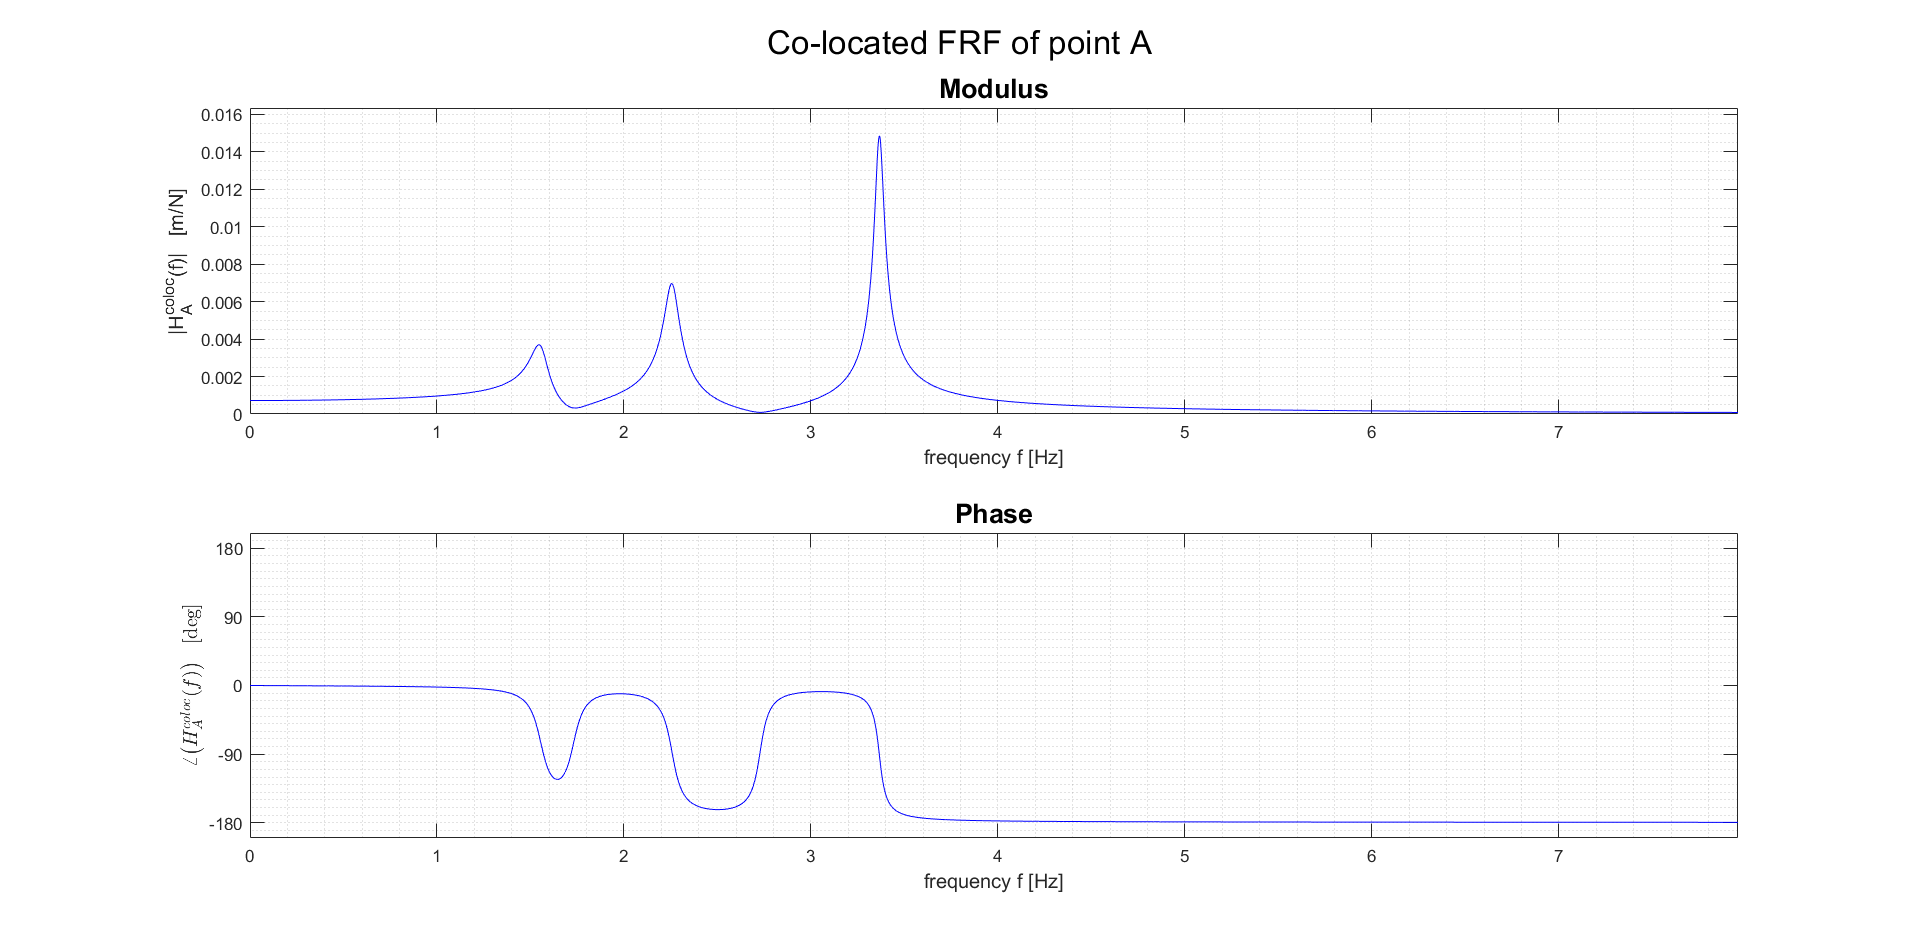
\includegraphics[scale=0.4]{co-located_a}
\end{figure}

\subsection{Co-located FRF of disc 2}

As a consequence of what we already said about the meaning of each element of the FRM, the requested co-located FRF is exactly the element $ H_{22} $ of the matrix:

\begin{figure}[h]
	\hspace{-70pt}
	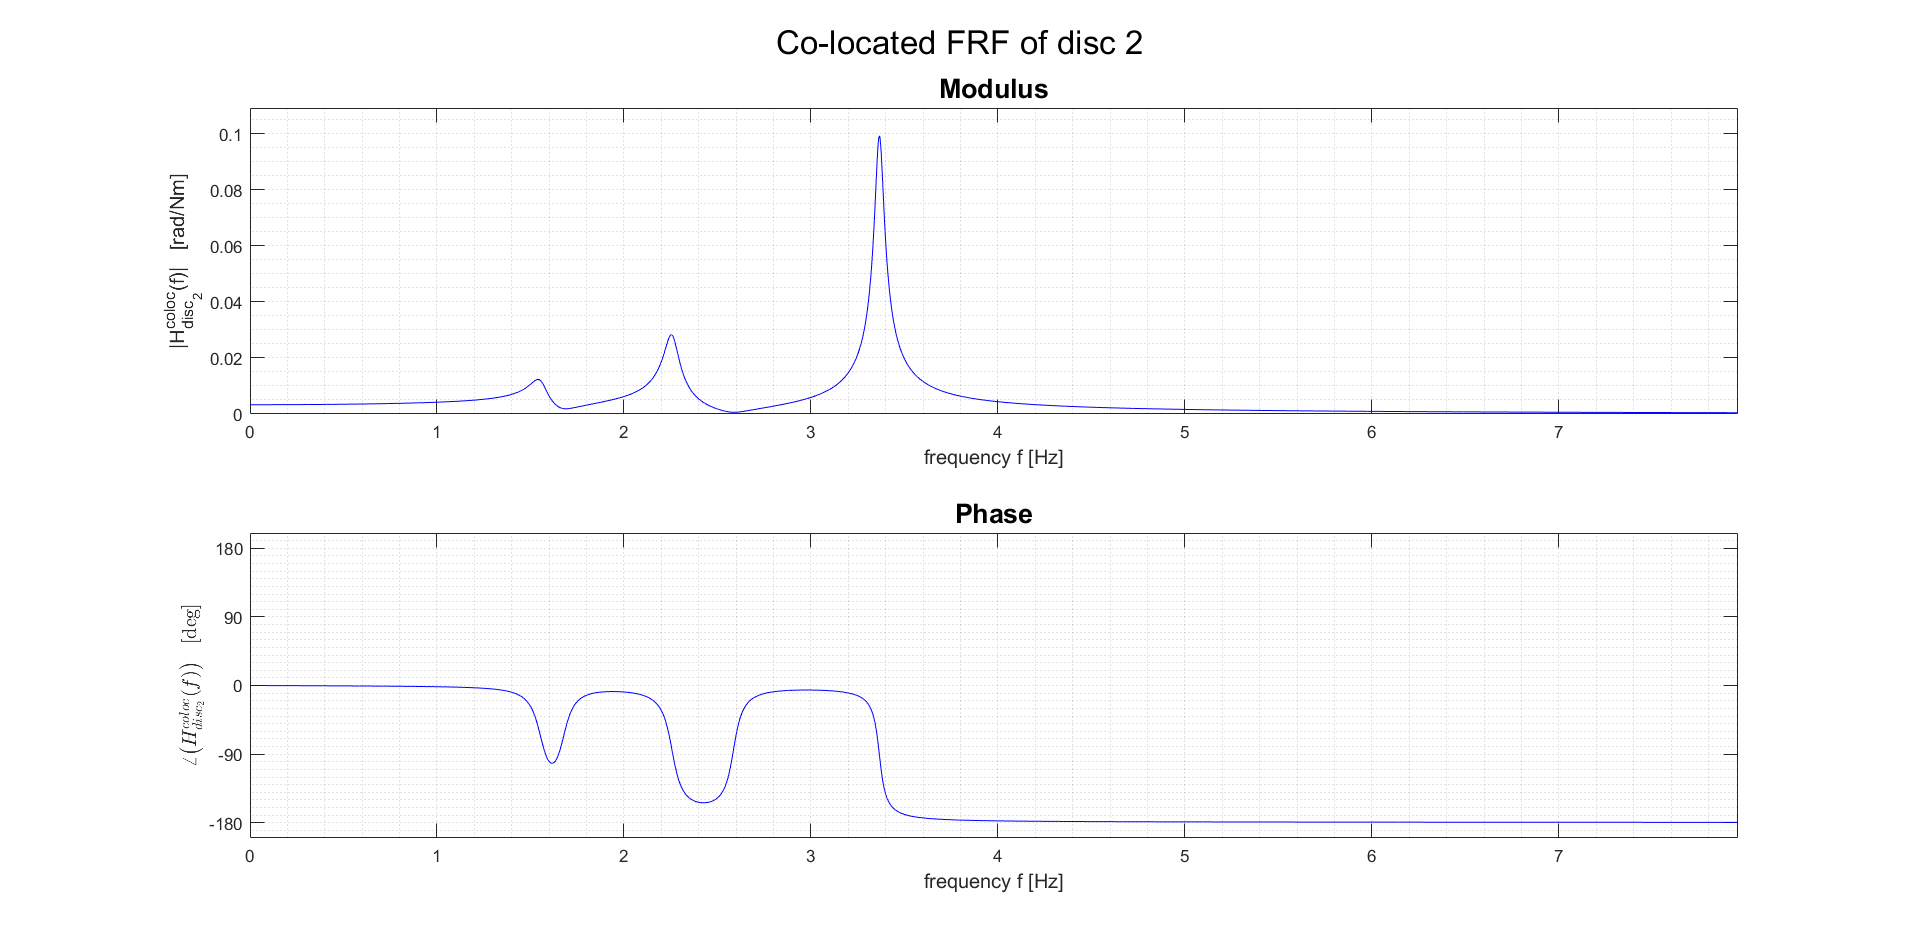
\includegraphics[scale=0.4]{co-located_disc2}
\end{figure}

\subsection{Complete time response of the system}

The complete time response is obtained summing the free response to the forced one. The initial conditions we're considering are those specified at \ref{subs:free_motion_given_initial_conditions}, so the free motion is the one we already computed $ \mathbf{u^{free}}(t) $. The forced motion is the response to the same horizontal force applied on point $ A $ that we considered so far, formed by two cosinusoidal components:

\[ F(t) = A_1 \, \cos(2 \pi f_1 \, t) + A_2 \, \cos(2 \pi f_2 \, t) \]

with $ A_1 = 15 \, \text{N} $, $ A_2 = 7 \, \text{N} $, $ f_1 = 1.5 \, \text{Hz} $, $ f_2 = 3.5 \, \text{Hz} $. The first step is to find the three FRFs for the case, so we're considering the case when the force is the generic $ F(t) = F_0 \, \cos(\Omega \, t) $. Starting from the equation of motion at \ref{eqn:motion} and proceeding as for the single-degree-of-freedom system, we have that

\[ \begin{split}
	& \mathbf{M^*} \, \ddot{\mathbf{u}} + \mathbf{C_{ray}} \, \dot{\mathbf{u}} +
		\mathbf{K^*} = \mathbf{Q_{u}} = \mathbf{\Lambda_F}^\textup{T} \, F(t) =
		\mathbf{\Lambda_F}^\textup{T} \, F_0 \, \cos(\Omega \, t) \\
	& \Rightarrow ~ \mathbf{D}(\Omega) \, \mathbf{\tilde{U}} \, e^{j \Omega \, t} =
		\mathbf{\Lambda_F}^\textup{T} \, F_0 \, e^{j \Omega \, t} ~ \Rightarrow ~
		\frac{\mathbf{\tilde{U}}}{F_0} =
		\mathbf{H}(\Omega) \, \mathbf{\Lambda_F}^\textup{T} =
		\mathbf{H_A}(\Omega)
\end{split} \]

Exploiting the superposition principle for the forced responses, the three time functions expressing the complete motion, in matricial form, are

\[ \begin{split}
	\mathbf{u}(t) & = \mathbf{u^{free}}(t) + \mathbf{u^{forced}}(t) = \\
								& = \sum_{i=1}^3 e^{-\alpha^{(i)} \, t} \, |\mathbf{U_d^{(i)}}|
									\Bigl(A^{(i)} \,
									\cos\bigl(\omega_\textup{d}^{(i)} \, t +
									\angle(\mathbf{U_d^{(i)}})\bigr) +
									B^{(i)} \,
									\sin\bigl(\omega_\textup{d}^{(i)} \, t +
									\angle(\mathbf{U_d^{(i)}})\bigr)\Bigr) + \\
								& ~~~ + |\mathbf{H_A(\omega_1)}| \, A_1 \, \cos\Bigl(\omega_1 \, t +
									\angle\bigl(\mathbf{H_A(\omega_1)}\bigr)\Bigr) +
									|\mathbf{H_A(\omega_2)}| \, A_2 \, \cos\Bigl(\omega_2 \, t +
									\angle\bigl(\mathbf{H_A(\omega_2)}\bigr)\Bigr)
\end{split} \]

where $ \omega_i = 2 \, \pi \, f_i \text{ , } i = 1,2 $. The corresponding three plots are reported here.

\begin{figure}[h]
	\hspace{-70pt}
	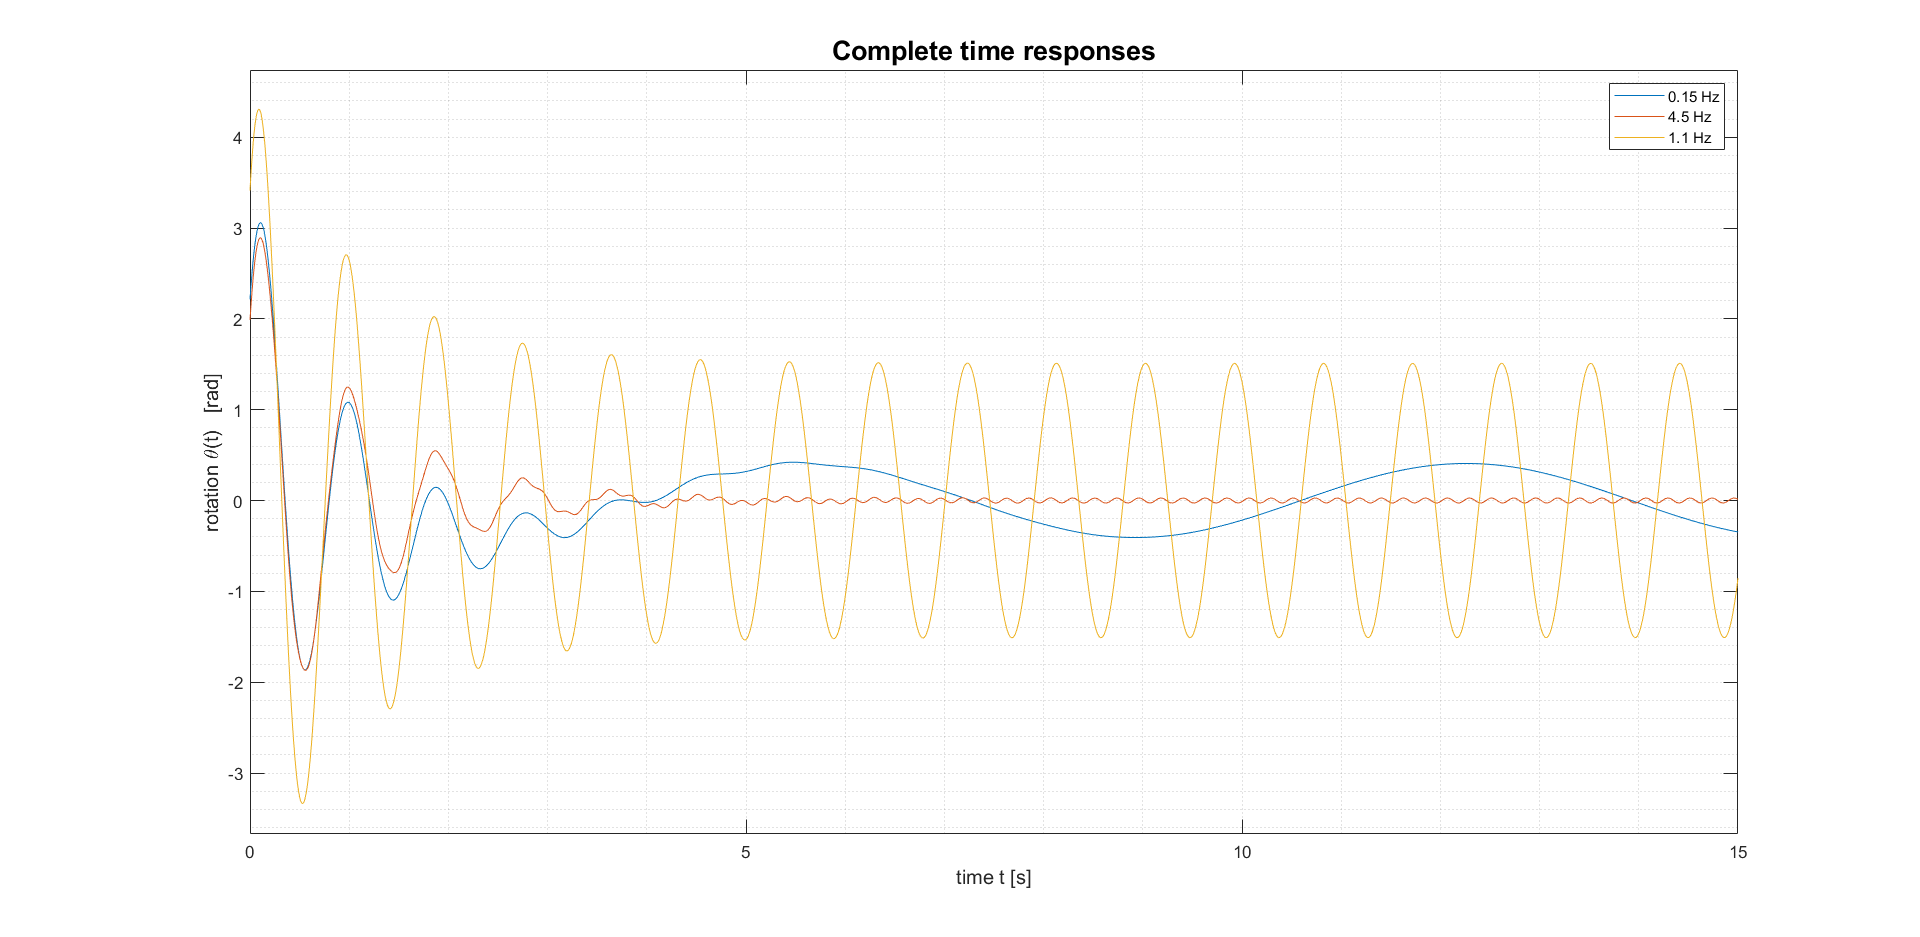
\includegraphics[scale=0.4]{complete_time_responses}
\end{figure}

\subsection{Forced response of the system (steady-state)}

The force we're now considering is still the one we assumed in our equation of motion, but this time its waveform is a triangular wave approximated to the 5\textsuperscript{th} harmonic:

\[
	F(t) = \frac{8}{\pi^2} \, \sum_{k=0}^4 (-1)^k
		\frac{\sin\bigl((2k + 1) \, 2 \pi f_0 \, t\bigr)}{(2k + 1)^2}
\]

We need to find the forced response of point $ A $, so we'll need to use the co-located FRF of paragraph \ref{subs:co-located_a} and evaluate it for the frequency values $ \omega^\textup{tr}_k = (2k + 1) \, 2 \pi f_0 \text{ , } k = 0,...,5 $, with $ f_0 = 0.75 \, \text{Hz} $, of the five harmonics of the force. The resulting horizontal displacement $ x_A $ for this forced motion is

\[
	x_A^\textup{forced}(t) = \frac{8}{\pi^2} \, \sum_{k=0}^4 (-1)^k \,
		|H^\textup{coloc}_A(\omega^\textup{tr}_k)| \,
		\frac{\sin\Bigl(\omega^\textup{tr}_k \, t +
		\angle\bigl(H^\textup{coloc}_A(\omega^\textup{tr}_k)\bigr)\Bigr)}{(2k + 1)^2}
\]

and the plots representing the force waveform and the forced time response are

\begin{figure}[h]
	\hspace{-70pt}
	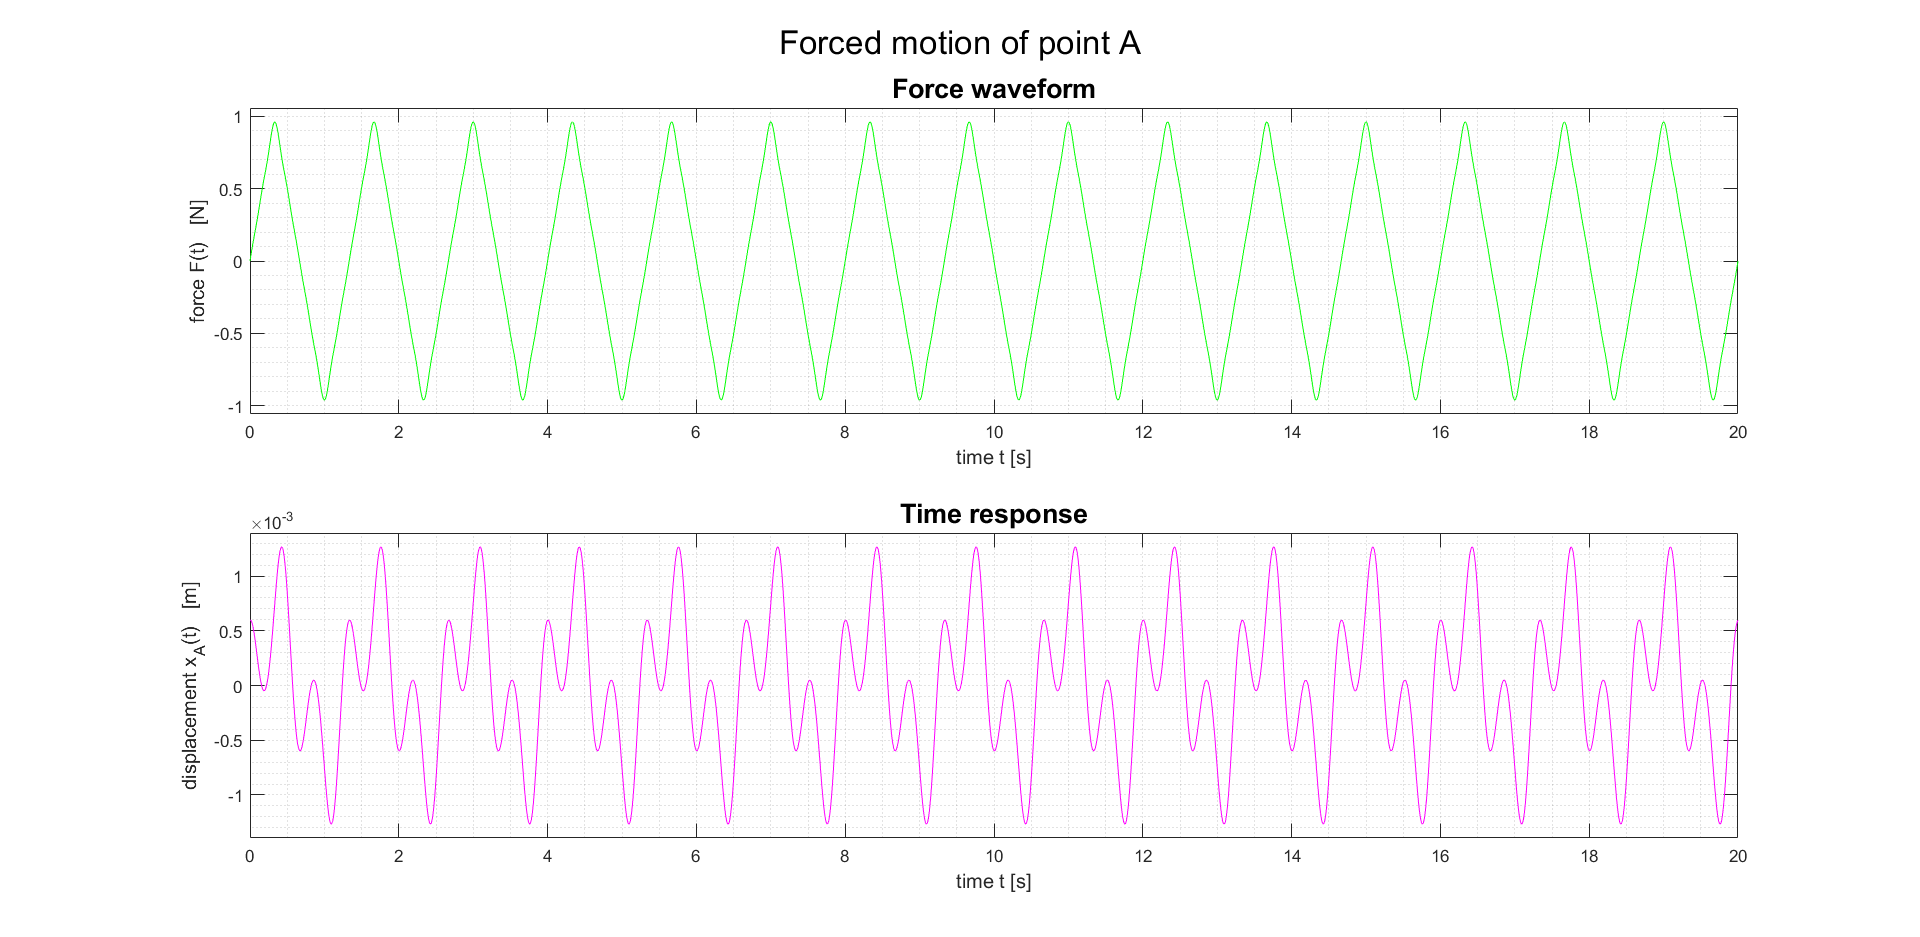
\includegraphics[scale=0.4]{forced_motion}
\end{figure}

Notice that the horizontal motion of point $ A $ is very small compared to the oscillation amplitude of the external harmonic excitation.


\section{Modal approach}

Finally, the system is analyzed using a modal superposition method to find the FRM and the co-located FRFs, and to compare the results obtained with the two procedures. The system damping is again assumed to be the Rayleigh damping.

\subsection{Equation of motion and Frequency Response Matrix}

The equation in modal coordinates is found thanks to the relation

\[ \mathbf{u} = \bm{\phi} \, \mathbf{q} \]

where $ \bm{\phi} $ is the modal matrix, equal to $ \mathbf{U_{und}} $ obtained gathering together the modeshapes for the undamped system in \ref{ssubs:undamped_parameters}. Applying this relation to the energy terms of \ref{ssubs:energy_terms}, what we have is

\[
	E_\textup{k} =
		\frac{1}{2} \, \dot{\mathbf{u}}^\textup{T} \, \mathbf{M^*} \, \dot{\mathbf{u}} =
		\frac{1}{2} \, \dot{\mathbf{q}}^\textup{T} \,	\bm{\phi}^\textup{T} \,
		\mathbf{M^*} \, \bm{\phi} \, \dot{\mathbf{q}}
\]

\[
	V = V_\textup{e} =
		\frac{1}{2} \, \mathbf{u}^\textup{T} \, \mathbf{K^*} \, \mathbf{u} =
		\frac{1}{2} \, \mathbf{q}^\textup{T} \,	\bm{\phi}^\textup{T} \,
		\mathbf{K^*} \, \bm{\phi} \, \mathbf{q}
\]

\[
	D = \frac{1}{2} \, \dot{\mathbf{u}}^\textup{T} \,	\mathbf{C_{ray}} \,
		\dot{\mathbf{u}} =
		\frac{1}{2} \, \dot{\mathbf{q}}^\textup{T} \,	\bm{\phi}^\textup{T} \,
		\mathbf{C_{ray}} \, \bm{\phi} \, \dot{\mathbf{q}}
\]

\[
	\delta W = \mathbf{Q_u}^\textup{T} \, \bm{\delta u} =
		\mathbf{Q_u}^\textup{T} \, \bm{\phi} \, \bm{\delta q}
\]

The equation of motion becomes

\[
	\underbrace{\bm{\phi}^\textup{T} \, \mathbf{M^*} \, \bm{\phi}}_
		{\substack{\text{modal mass matrix} \\
		\text{$ \mathbf{M_q} $}}} \, \ddot{\mathbf{q}} +
		\underbrace{\bm{\phi}^\textup{T} \, \mathbf{C_{ray}} \,	\bm{\phi}}_
		{\substack{\text{modal damping matrix} \\
		\text{$ \mathbf{C_q} $}}} \, \dot{\mathbf{q}} +
		\underbrace{\bm{\phi}^\textup{T} \, \mathbf{K^*} \, \bm{\phi}}_
		{\substack{\text{modal stiffness matrix} \\
		\text{$ \mathbf{K_q} $}}} \, \mathbf{q} =
		\underbrace{\bm{\phi}^\textup{T} \, \mathbf{Q_u}}_
		{\substack{\text{modal forces vector} \\
		\text{$ \mathbf{F_q} $}}}
\]

These form a system of $ N $ equations, each describing the motion of a single-degree-of-freedom system:

\[ \begin{cases}
	m^{(1)} \, \ddot{q}^{(1)} + c^{(1)} \, \dot{q}^{(1)} + k^{(1)} \, q^{(1)} =
		F_\textup{q}^{(1)} \\
	m^{(2)} \, \ddot{q}^{(2)} + c^{(2)} \, \dot{q}^{(2)} + k^{(2)} \, q^{(2)} =
		F_\textup{q}^{(2)} \\
	m^{(3)} \, \ddot{q}^{(3)} + c^{(3)} \, \dot{q}^{(3)} + k^{(3)} \, q^{(3)} =
		F_\textup{q}^{(3)}
\end{cases} \]

where $ m^{(i)} $, $ c^{(i)} $ and $ k^{(i)} \text{ , } i = 1,2,3 $ are the element $ M_{\textup{q}_{ii}} $, $ C_{\textup{q}_{ii}} $ and $ K_{\textup{q}_{ii}} $ of the modal mass, damping and stiffness matrix respectively. Note in particular that, since we assumed the system to be damped with Rayleigh damping, we don't run the risk of having a full modal damping matrix, but we're rather ending up with a diagonal $ \mathbf{C_q} $. Since we decomposed the system into a superposition of $ N $ simple oscillatory systems, we expect the elements on the diagonal of the modal Frequency Response Matrix $ \mathbf{H_q}(\Omega) $ to be the FRF for a single-degree-of-freedom system, with its own damping factor $ \alpha^{(i)} = \frac{c^{(i)}}{2 \, m^{(i)}} $, natural frequency $ \omega_\textup{n}^{(i)} = \sqrt{\frac{k^{(i)}}{m^{(i)}}} $, damped natural frequency $ \omega_\textup{d}^{(i)} = \sqrt{(\omega_\textup{n}^{(i)})^2 - (\alpha^{(i)})^2} $ and all the parameters that we already got in \ref{ssubs:damped_parameters}, exhibiting a single peak in the magnitude diagram and a single jump from $ 0 $ to $ -\pi $ in the phase diagram, both in correspondence with the damped natural frequency. The $ N $ FRFs on the diagonal are in fact given by

\[
	H_q(\Omega) = \frac{\tilde{Q}^{(i)}(\Omega)}{F_{\textup{q}_0}^{(i)}} =
	\frac{1}{-m^{(i)} \, \Omega^2 + j c^{(i)} \, \Omega + k^{(i)}}
\]

which are found solving the differential equations considering $ F_\textup{q}^{(i)} = F_{\textup{q}_0}^{(i)} \, \cos(\Omega t) $. On the other hand, we expect the extra-diagonal elements  to be equal to zero, as each  mode is decoupled from the others. However, Matlab consider those terms as greater than zero, but since they're in the order of $ 10^{-17} $ we set them directly to zero, concluding they're due to numerical errors. The modulus and phase plots are the following:

\clearpage

\begin{figure}
	\hspace{-70pt}
	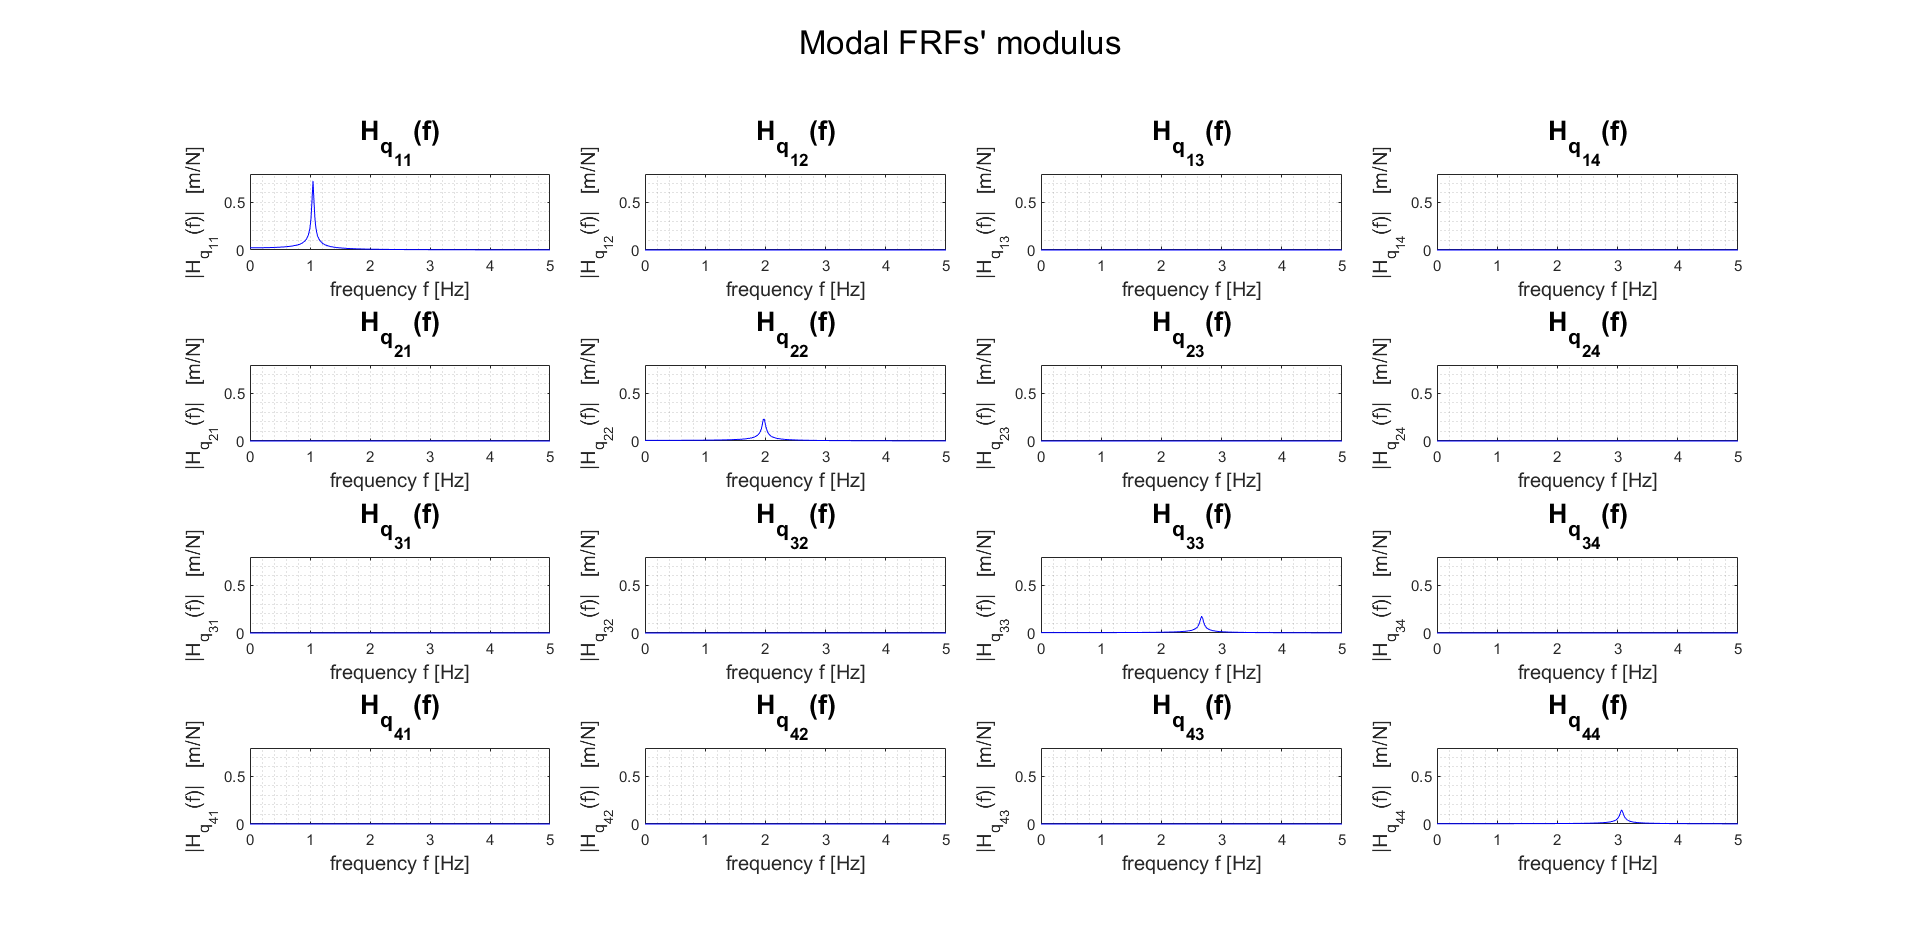
\includegraphics[scale=0.4]{modal_frfs_modulus}
\end{figure}

\begin{figure}[H]
	\hspace{-70pt}
	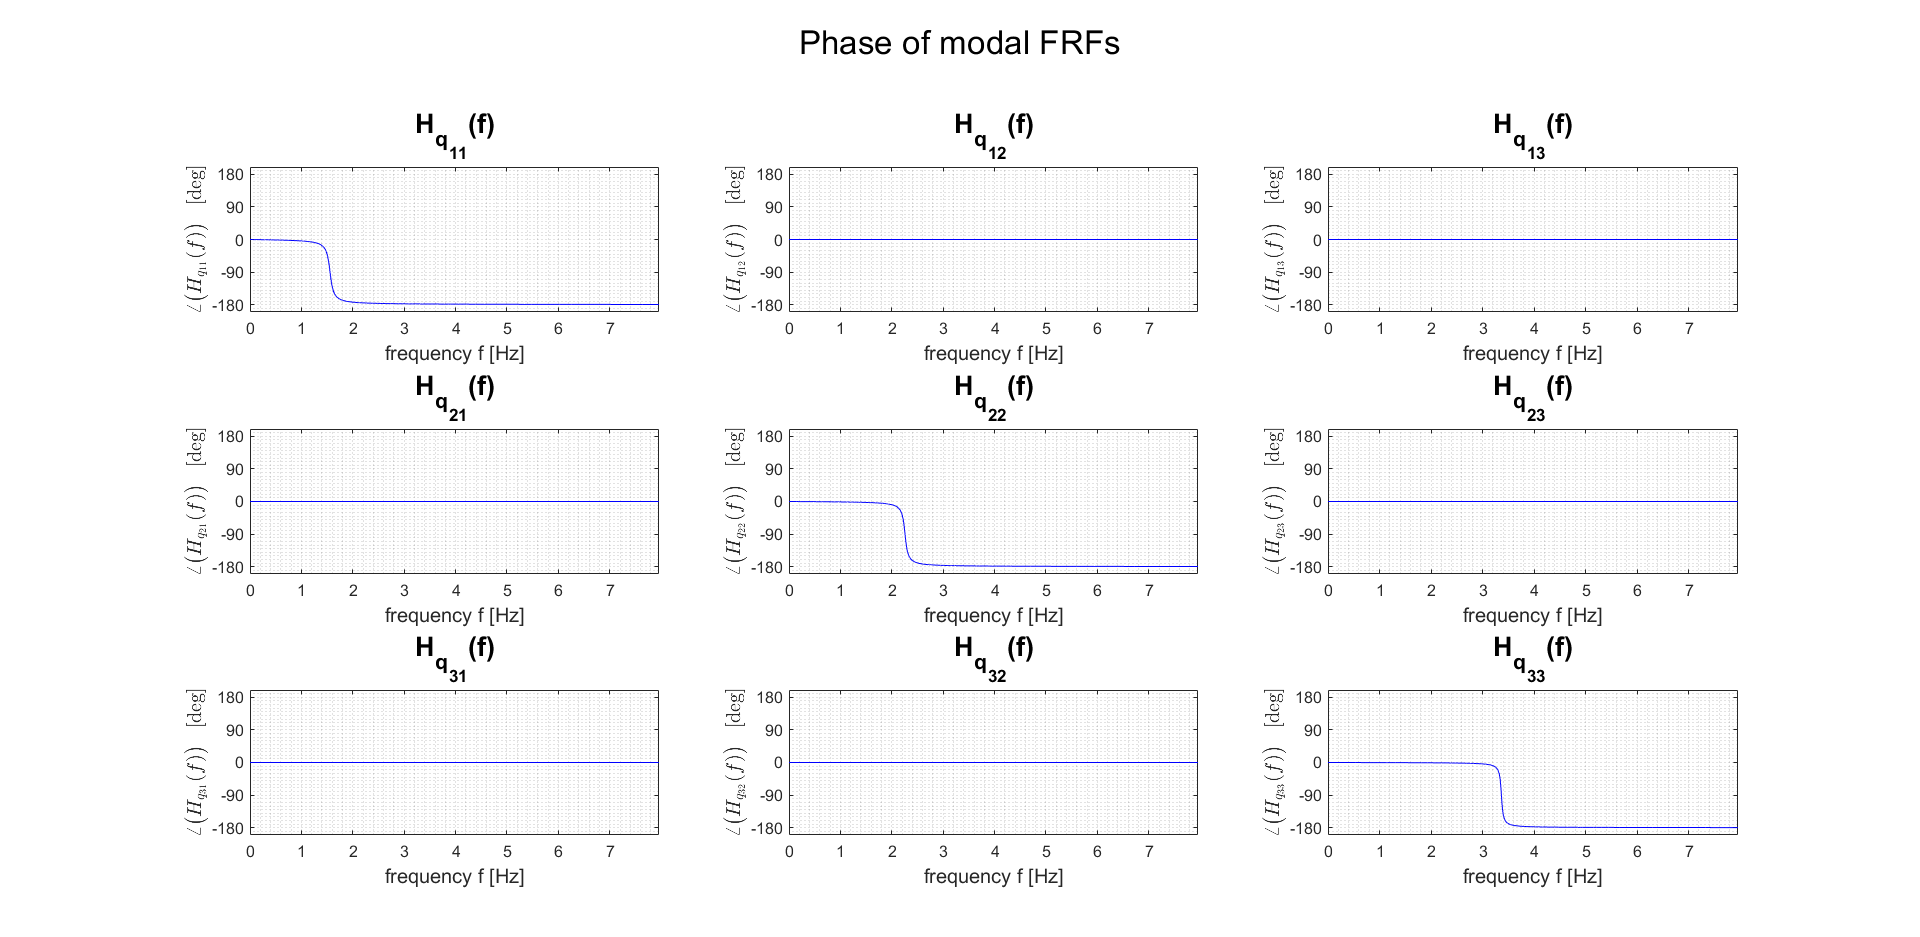
\includegraphics[scale=0.4]{modal_frfs_phase}
\end{figure}

Notice that the oscillation following the first mode is very small in terms of amplitude with respect to the one following the other two modes.

\clearpage

\subsection{Co-located FRF of point A}

The co-located FRF of point $ A $ is now reconstructed using the modal approach, and compared to the one previously found. The reconstruction passes through finding a new Jacobian for the force:

\[
	\mathbf{\Lambda_{q_F}} = \mathbf{\Lambda_F} \, \bm{\phi}
\]

Then the operations to find the FRF are the same as for \ref{subs:co-located_a}:

\[
	H^\textup{coloc}_{\textup{q}_A}(\Omega) =
		\mathbf{\Lambda_{q_F}} \, \mathbf{H}(\Omega) \,
		\mathbf{\Lambda_{q_F}}^\textup{T}
\]

As we may see in the following picture, the two approaches lead to the same plots:

\begin{figure}[h]
	\hspace{-70pt}
	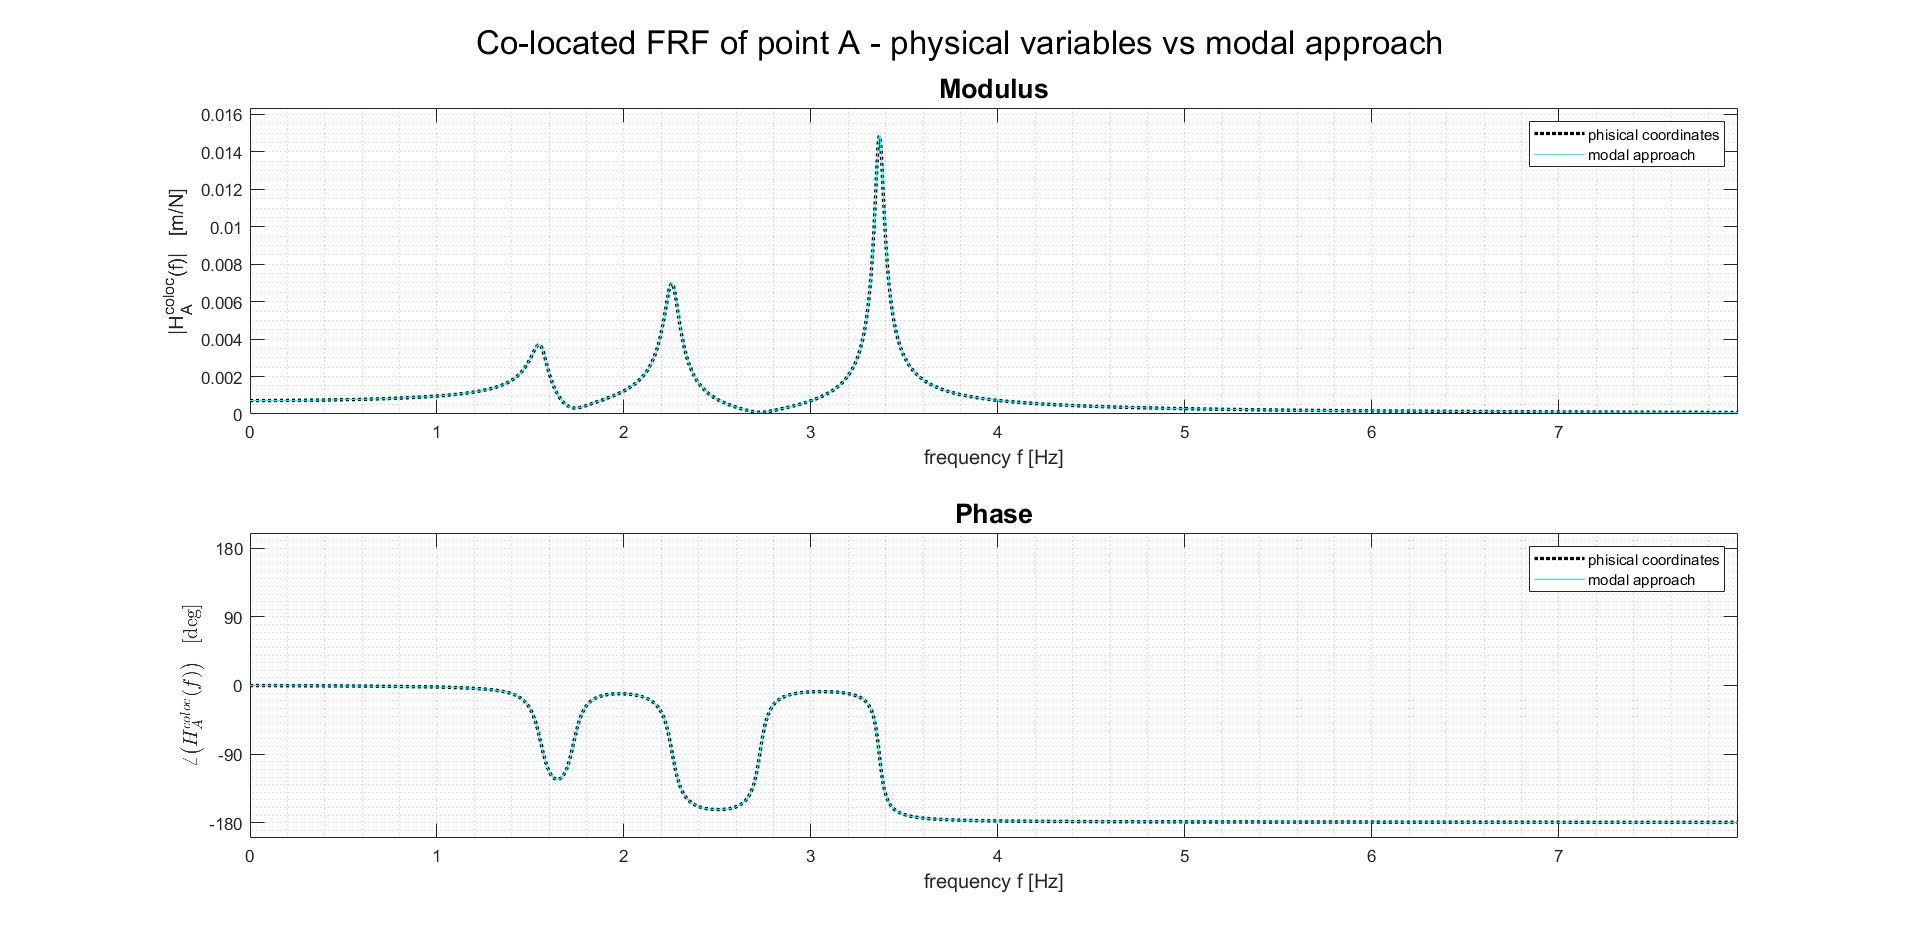
\includegraphics[scale=0.4]{co-located_a_physical_vs_modal}
\end{figure}

\clearpage

\subsection{Co-located FRF of disc 2}

As a final step, we do the same for the co-located FRF of disc 2:

\[
	\mathbf{\Lambda_{q_\tau}} = \mathbf{\Lambda_\tau} \, \bm{\phi} ~ \Rightarrow ~
		H^\textup{coloc}_{\textup{q}_{disc_2}}(\Omega) =
		\mathbf{\Lambda_{q_\tau}} \, \mathbf{H}(\Omega) \,
		\mathbf{\Lambda_{q_\tau}}^\textup{T}
\]

where the Jacobian $ \mathbf{\Lambda_\tau} $, since this FRF is the co-located FRF found in the FRM of \ref{subs:frm} for the second independent variable, is equal to $ [0, 1, 0] $. Again, the FRFs found by means of physical coordinates and of modal ones perfectly coincide:

\begin{figure}[h]
	\hspace{-70pt}
	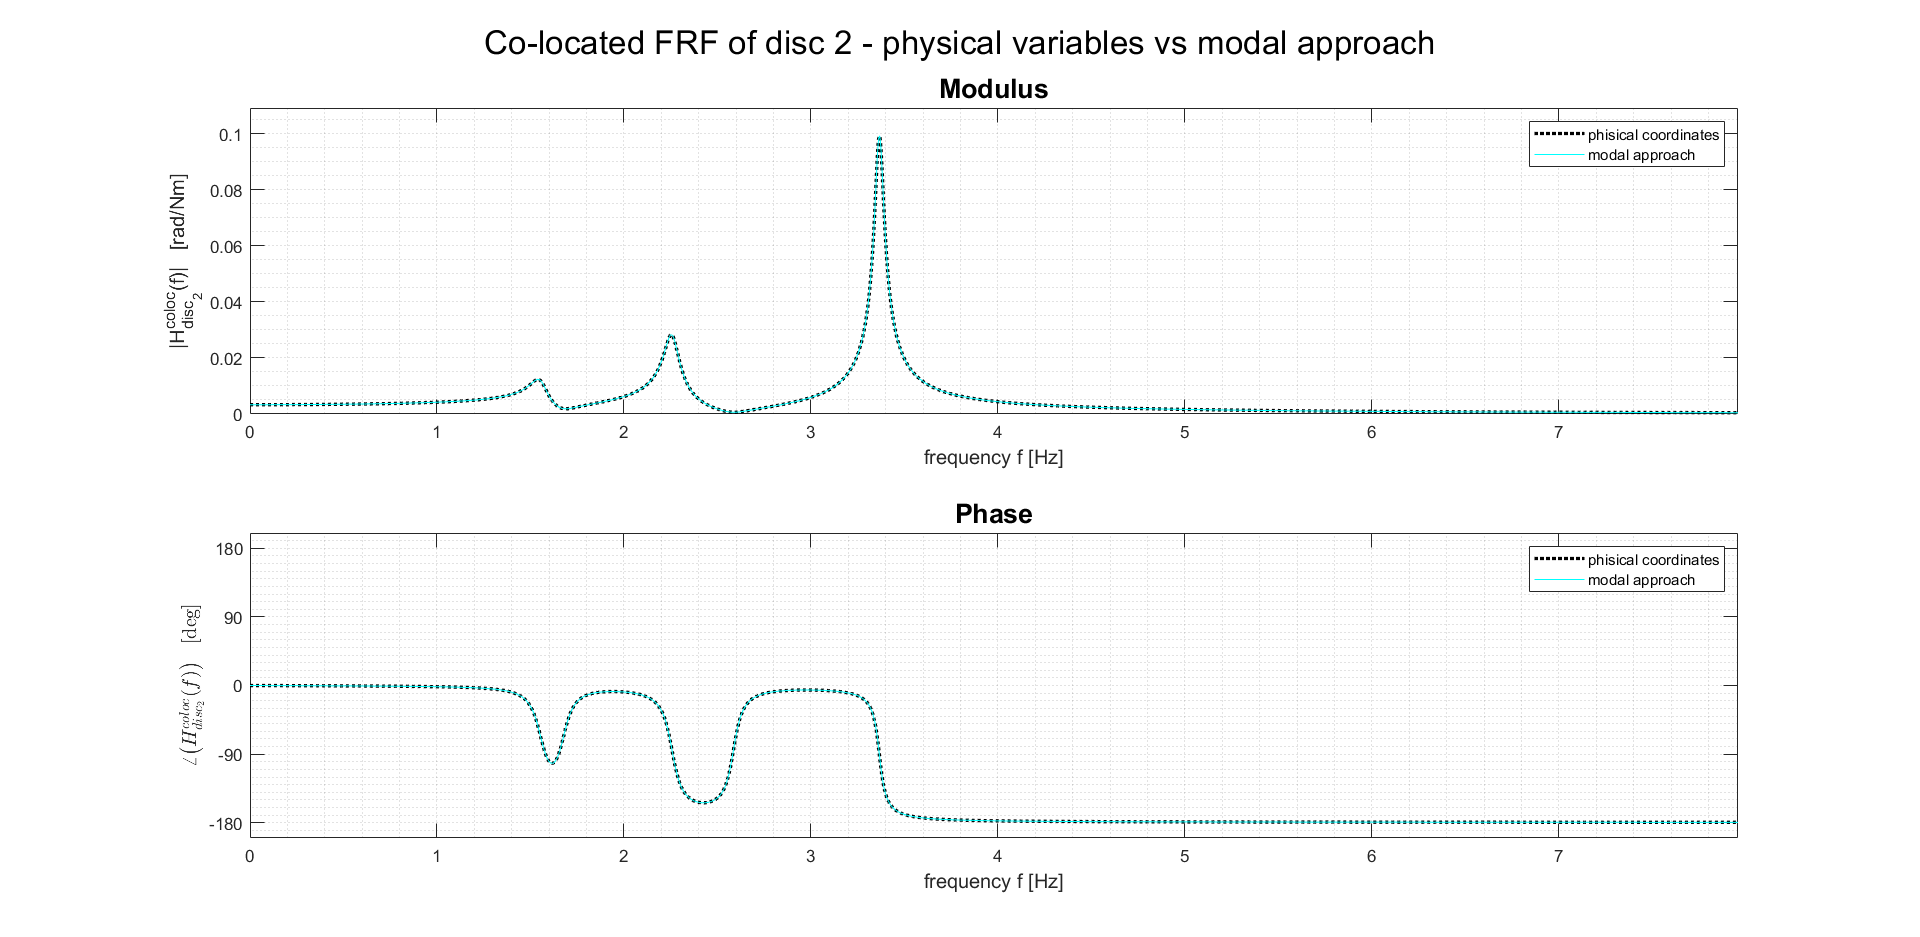
\includegraphics[scale=0.4]{co-located_disc2_physical_vs_modal}
\end{figure}


\end{document}
